\documentclass[preprint, onecolumn, amsmath, amssymb, aps, floatfix]{revtex4-2}

% --- Packages ---
\usepackage[utf8]{inputenc}
\usepackage{graphicx}
\usepackage{booktabs}
\usepackage{bm}
\usepackage{hyperref}
\usepackage{amsthm}
\usepackage{amsmath}
\usepackage{amssymb}
\usepackage{tikz}
\usepackage{subcaption}
% longtable omitted -- revtex4-2 provides its own longtable support
\usepackage{xcolor}
\usepackage[capitalize,noabbrev]{cleveref}

\usetikzlibrary{graphs, shapes.geometric, arrows.meta}

% --- Figure path ---
\graphicspath{{figures/}}

% --- Custom environments ---
\newtheorem{keyresult}{Key Result}
\newtheorem{convention}{Convention}
\newtheorem{correspondence}{Correspondence}

% --- cleveref formats for custom environments ---
\crefname{keyresult}{Key Result}{Key Results}
\Crefname{keyresult}{Key Result}{Key Results}

% --- Custom operators ---
\DeclareMathOperator{\rank}{rank}
\DeclareMathOperator{\im}{im}
\DeclareMathOperator{\diag}{diag}
\DeclareMathOperator{\tr}{tr}
\DeclareMathOperator{\sgn}{sgn}
\DeclareMathOperator{\perm}{perm}
\DeclareMathOperator{\Skew}{skew}

% --- Shortcuts ---
\newcommand{\R}{\mathbb{R}}
\newcommand{\Z}{\mathbb{Z}}
\newcommand{\calP}{\mathcal{P}}
\newcommand{\calI}{\mathcal{I}}
\newcommand{\calQ}{\mathcal{Q}}
\newcommand{\calH}{\mathcal{H}}

\begin{document}

% ===================================================================
% FRONT MATTER
% ===================================================================
\title{Topological Deep Learning and Artificial Spin Ice:\\ A Mathematical Correspondence and Neural Sampling Proposal}
\author{Carl Merrigan}
\author{Cristiano Nisoli}
\author{Claude Opus-4.6}
\date{\today}

\begin{abstract}
This document has two parts, both preliminary.
%
The first part works out the mathematical correspondence between the
simplicial-complex formalism used in Topological Deep Learning (TDL)---boundary
operators, Hodge Laplacians, cochains---and Nisoli's charge framework for
artificial spin ice (ASI).  The operators turn out to be identical, not
merely analogous: the same $B_1$, $L_0$, $L_1^{\text{down}}$ that appear
in TDL message passing are exactly the objects in the ASI charge and
Hamiltonian theory.  We spell out the dictionary (six ``key results''
connecting $S_{vv'}$, topological charge, the Hodge decomposition, and the
Hamiltonian to TDL quantities) and present a counting table showing how
much the directed-cycle constraint reduces the reachable ice-state count
below the topological bound $2^{\beta_1}$---by up to five orders of
magnitude across the lattice zoo.
%
The second part sketches an idea for future application: using recent
work on variational autoregressive networks (VAN), message-passing VAN
(MPVAN), and the EIGN edge-level GNN architecture to build neural samplers
for spin ice configurations.  We outline two complementary modes---loop-basis
sampling (Mode~A, guaranteed ice-rule compliance) and direct-edge sampling
(Mode~B, finite temperature)---and write down the layer update equations
and training objectives.  These architectures are at a preliminary concept
stage; there are many implementation and training details still to be
worked out, and we expect the design to evolve considerably.
We share this document to invite critical review of the ideas before
investing further in implementation.
\end{abstract}

\maketitle

% ===================================================================
% SECTION 1: INTRODUCTION
% ===================================================================
\section{Introduction}
\label{sec:intro}

This document works through the mathematical correspondence between two
bodies of theory that, at first glance, belong to entirely different fields:

\begin{itemize}
  \item \textbf{Topological Deep Learning (TDL)}---the framework of simplicial
    complexes, boundary operators, Hodge Laplacians, and cochains that
    generalizes graph neural networks to higher-order
    structures~\cite{hajij2023topological,papillon2024architectures}.
  \item \textbf{Artificial Spin Ice (ASI) graph theory}---the charge
    framework~\cite{nisoli2020} for frustrated lattice systems, which describes
    spin configurations, topological charges, ice rules, and entropic
    interactions using the combinatorial Laplacian and its pseudoinverse.
\end{itemize}

The connection turns out to be structural, not analogical: the same
operator---the graph Laplacian~$L_0$ and its edge-level counterpart
$L_1^{\text{down}} = B_1^T B_1$---governs both the entropic interactions
between topological charges in spin ice \emph{and} the message-passing
dynamics in graph neural networks.  The first part of this document
(Secs.~\ref{sec:notation}--\ref{sec:hamiltonian}) spells out the dictionary
in detail, deriving six ``key results'' that translate objects from the ASI
charge framework---$S_{vv'}$, topological charge, Coulomb classes, ice
manifold, Hodge decomposition, Hamiltonian---into standard TDL quantities.
A particular focus is the counting table (\cref{sec:counting_table}), which
tracks how much the directed-cycle constraint reduces the reachable ice-state
count below the topological bound $2^{\beta_1}$.

The second part (\cref{sec:outlook}) sketches an idea for where this
correspondence might lead: neural samplers for spin ice configurations,
built by combining three recent developments from the machine learning
literature.  Variational autoregressive networks
(VANs)~\cite{wu2019variational} showed that autoregressive neural networks
can learn to sample from Boltzmann distributions of classical spin systems,
replacing MCMC with single-pass generation.  The message-passing VAN
(MPVAN)~\cite{ma2024mpvan} demonstrated that incorporating the Hamiltonian's
coupling structure directly into message-passing weights improves sampling
quality on frustrated Ising models.  And the EIGN
architecture~\cite{fuchsgruber2025} introduced edge-level message passing
that respects orientation equivariance, using operator channels built from
$B_1$ and $|B_1|$.  \Cref{sec:outlook} sketches how these three ideas might
combine into two complementary sampling architectures for ASI---one operating
in the loop basis (Mode~A), the other sampling edges directly (Mode~B).
These are preliminary designs; there are likely many implementation and
training details that will need to be worked out, and the architectures may
change substantially as we learn more.

The ice manifold (the degenerate ground-state manifold of a frustrated spin
ice) is structurally governed by $\ker(B_1)$---either as the ice manifold
itself (for even-degree vertices) or as the space of fluctuations within it
(for odd-degree vertices).  The dimension of this space, its combinatorial
density (Pauling entropy), and its spectral structure all vary across lattice
types in ways that ASI physics has characterized in detail.  A particular
focus of the formalism sections is the relationship between $\beta_1$ and
the degeneracy of the ice manifold: $\beta_1$ sets an upper bound of
$2^{\beta_1}$ on the reachable ice states per charge sector
(\cref{sec:loop_basis}), but the actual count is controlled by a
\textbf{directed-cycle constraint} that can reduce it by orders of magnitude
(\cref{sec:counting_table}).  This distinction matters for neural sampling,
where training difficulty depends on the reachable state count, not on
$\beta_1$ alone.

The remainder of this document is organized as follows.
\Cref{sec:notation} establishes notation and the simplicial complex setup.
\Cref{sec:S_matrix,sec:charge} derive the correspondence for the
$S_{vv'}$ matrix and the topological charge.
\Cref{sec:coulomb} develops the Coulomb class structure, ice manifold
parameterization, and the counting table.
\Cref{sec:hodge} presents the Hodge decomposition, and \cref{sec:hamiltonian}
connects the spin-ice Hamiltonian to the lower Hodge Laplacian.
\Cref{sec:outlook} sketches the two neural-sampling architectures, and
\cref{sec:summary} summarizes.

% ===================================================================
% SECTION 2: NOTATION & SETUP
% ===================================================================
\section{Notation and Setup}
\label{sec:notation}

\subsection{The graph}
\label{sec:graph}

We work with a \textbf{connected} simple undirected graph $G = (V, E)$ with
$n_0 = |V|$ vertices and $n_1 = |E|$ edges. Connectivity means $\beta_0 = 1$
(one connected component); the graph Laplacian $L_0$ has exactly one zero
eigenvalue with eigenvector $\mathbf{1}$, and $\rank(B_1) = n_0 - 1$. All
ASI lattices we consider are connected, planar (or toroidal under periodic
boundary conditions), with vertex coordination numbers $z_v \in \{2,3,4\}$.

To define incidence matrices and boundary operators, we equip each edge with
a \textbf{reference orientation}: for edge~$e$ connecting vertices~$u$
and~$v$, we designate one vertex as the tail (source) and the other as the
head (target). The physics does not depend on this choice---changing the
orientation of an edge negates the corresponding column of $B_1$ and the
corresponding component of any 1-cochain, leaving all observables invariant.

\begin{convention}[Reference Orientation]
For lattices on $\Z^2$, we orient horizontal edges left$\to$right and
vertical edges bottom$\to$top. For edges not aligned with axes, we orient
from the vertex with smaller index to the vertex with larger index.
\end{convention}

\subsection{Simplicial complex}
\label{sec:simplicial}

A simplicial complex $X$ built on $G$ extends the graph to include
higher-dimensional cells:
\begin{itemize}
  \item \textbf{0-simplices (vertices):} the $n_0$ vertices of $G$
  \item \textbf{1-simplices (edges):} the $n_1$ oriented edges of $G$
  \item \textbf{2-simplices (faces):} $n_2$ oriented filled polygonal faces
\end{itemize}

The vertices and edges are given by the graph, but the \textbf{faces are a
modeling choice}. Morrison, Nelson \& Nisoli~\cite{morrison2013} define a
\emph{minimal loop} as a closed chain of edges that does not contain vertices
in its interior---equivalently, the faces of the planar embedding. These
minimal loops are the fundamental objects in ASI frustration theory and the
natural candidates for 2-cells. Given the set of all minimal loops, we
consider two bracketing strategies:

\begin{table}[h]
\centering
\caption{Face-filling strategies and their effect on $\beta_1$.}
\label{tab:face_strategies}
\begin{tabular}{llll}
\toprule
\textbf{Strategy} & $n_2$ & $L_1^{\text{up}}$ & \textbf{Effect on $\beta_1$} \\
\midrule
Fill all faces & Maximal & Nonzero & Minimal $\beta_1$ \\
Fill no faces  & $0$     & $0$     & Maximal $\beta_1 = n_1 - n_0 + 1$ \\
\bottomrule
\end{tabular}
\end{table}

\textbf{Boundary conditions} also have a dramatic effect on $\beta_1$.
Consider the $3\times 3$ square lattice ($n_0=9$, $n_1^{\text{per}}=18$,
$n_1^{\text{open}}=12$):

\begin{table}[h]
\centering
\caption{Boundary condition effects on the $3\times 3$ square lattice.}
\label{tab:bc_effects}
\begin{tabular}{lccc}
\toprule
\textbf{Property} & \textbf{Periodic (torus)} & \textbf{Open (planar)} \\
\midrule
$n_0$ (vertices)                   & 9   & 9 \\
$n_1$ (edges)                      & 18  & 12 \\
$n_2$ (faces, all filled)          & 9   & 4 \\
$\chi = n_0 - n_1 + n_2$          & 0   & 1 \\
$\beta_0$                          & 1   & 1 \\
$\beta_2$                          & 1   & 0 \\
$\beta_1$ (all faces filled)       & \textbf{2}  & \textbf{0} \\
$\beta_1$ (no faces filled)        & \textbf{10} & \textbf{4} \\
\bottomrule
\end{tabular}
\end{table}

On the periodic torus, $\beta_1 = 2$ with all faces filled corresponds to the
two independent winding modes (horizontal and vertical) of $H_1(\mathbb{T}^2)
\cong \Z^2$. All three horizontal row-loops are \emph{homologous}---they
differ by the boundary of the faces between them---and similarly for the three
vertical column-loops. In the open case, every cycle on the planar patch bounds
a region of faces, so $\beta_1 = 0$ with all faces filled. This makes boundary
conditions a critical parameter: \textbf{periodic BCs guarantee a nonzero
$\beta_1$ floor} (at least~2 for a torus).

\subsection{Notation correspondence table}
\label{sec:notation_table}

\Cref{tab:notation} provides a dictionary between TDL and Nisoli notation.

\begin{table*}[t]
\centering
\caption{Notation correspondence between TDL and Nisoli's ASI charge framework.}
\label{tab:notation}
\small
\begin{tabular}{llll}
\toprule
\textbf{Object} & \textbf{TDL Notation} & \textbf{Nisoli Notation} & \textbf{Notes} \\
\midrule
Undirected graph & $G = (V,E)$ & $G$ with $N_v$ vertices, $N_l$ edges & $n_0 = N_v$, $n_1 = N_l$ \\
Adjacency matrix & $A$ or $A_{0,\text{down}}$ & $A_{vv'}$ & Symmetric, binary \\
Degree / coordination & $\deg(v)$, degree matrix $D$ & $z_v$ & $D_{vv} = z_v$ \\
Signed incidence & $B_1$ ($n_0 \times n_1$) & (implicit in $S_{vv'}$) & $[B_1]_{v,e} = \pm 1$ \\
Edge-face incidence & $B_2$ ($n_1 \times n_2$) & (not used by Nisoli) & Hodge decomposition \\
Edge signal / 1-cochain & $\mathbf{f} \in C^1(X;\R)$ & $\sigma_l$ (spin on edge) & $\sigma_e \in \{+1,-1\}$ \\
Vertex signal / 0-cochain & $\mathbf{h} \in C^0(X;\R)$ & $\varphi_v$ (entropic field) & \\
Graph Laplacian & $L_0 = B_1 B_1^T$ & $\hat{L}_{vv'} = z_v\delta_{vv'} - A_{vv'}$ & $L_0 = D - A$ \\
Lower Hodge Laplacian & $L_1^{\text{down}} = B_1^T B_1$ & (in energy: $\bm\sigma^T L_1^{\text{down}}\bm\sigma$) & Acts on $\R^{n_1}$ \\
Upper Hodge Laplacian & $L_1^{\text{up}} = B_2 B_2^T$ & (not used by Nisoli) & Requires 2-cells \\
Full Hodge 1-Laplacian & $L_1 = L_1^{\text{down}} + L_1^{\text{up}}$ & --- & Central for oversmoothing \\
Antisymmetric spin matrix & --- & $S_{vv'} = A^{\text{dir}}_{vv'} - A^{\text{dir}}_{v'v}$ & See \cref{sec:S_matrix} \\
Topological charge & $(B_1\bm\sigma)_v$ & $Q_v[S] = \sum_{v'} S_{v'v}$ & See \cref{sec:charge} \\
Ice manifold & $\ker(B_1) \cap \{\pm 1\}^{n_1}$ & $\calI = \{\sigma: Q_v = 0\;\forall v\}$ & See \cref{sec:ice_manifold} \\
Harmonic subspace & $\ker(L_1)$, dim $= \beta_1$ & Topological winding modes & See \cref{sec:hodge} \\
Coulomb class & $C_{\mathbf{q}}$ & Charge sector & See \cref{sec:coulomb_classes} \\
Pauling entropy & $s(G)$ & Entropy per vertex of $\calI$ & $s = \ln|\calI|/n_0$ \\
\bottomrule
\end{tabular}
\end{table*}

\subsection{Boundary operators}
\label{sec:boundary_ops}

The \textbf{vertex-edge incidence matrix} $B_1$ ($n_0 \times n_1$) is defined
by: for edge $e$ oriented from vertex $u$ (tail) to $v$ (head),
\begin{equation}
  [B_1]_{w,e} = \begin{cases}
    +1 & \text{if } w = v \text{ (head of } e\text{)} \\
    -1 & \text{if } w = u \text{ (tail of } e\text{)} \\
    0  & \text{otherwise.}
  \end{cases}
  \label{eq:B1def}
\end{equation}

The \textbf{edge-face incidence matrix} $B_2$ ($n_1 \times n_2$) is defined
by: for face $f$ with oriented boundary cycle,
\begin{equation}
  [B_2]_{e,f} = \begin{cases}
    +1 & \text{if } e \in \partial f \text{ with consistent orientation} \\
    -1 & \text{if } e \in \partial f \text{ with opposite orientation} \\
    0  & \text{if } e \notin \partial f.
  \end{cases}
  \label{eq:B2def}
\end{equation}

The fundamental chain complex property is
\begin{equation}
  B_1 B_2 = 0,
  \label{eq:chain}
\end{equation}
which states that ``the boundary of a boundary is zero.'' Equivalently, the
divergence of a curl is zero, or $\im(B_2) \subseteq \ker(B_1)$.

% ===================================================================
% SECTION 3: THE S MATRIX
% ===================================================================
\section{The \texorpdfstring{$S_{vv'}$}{S} Matrix as Incidence Times Spin Configuration}
\label{sec:S_matrix}

\subsection{Nisoli's definition}

In Nisoli~\cite{nisoli2020}, a spin configuration on a graph assigns to each
edge a direction. This is encoded in the directed adjacency matrix:
\begin{equation}
  A^{\text{dir}}_{vv'} = \begin{cases}
    1 & \text{if the spin on edge } \{v,v'\} \text{ points } v \to v' \\
    0 & \text{otherwise.}
  \end{cases}
  \label{eq:Adir}
\end{equation}
For each undirected edge $\{v,v'\}$, exactly one of $A^{\text{dir}}_{vv'}$ and
$A^{\text{dir}}_{v'v}$ equals~1. Nisoli defines the antisymmetric matrix:
\begin{equation}
  S_{vv'} = A^{\text{dir}}_{vv'} - A^{\text{dir}}_{v'v},
  \label{eq:Sdef}
\end{equation}
satisfying $S_{vv'} = -S_{v'v} \in \{-1, 0, +1\}$, with $S_{vv'} = 0$ for
non-adjacent vertices.

\subsection{TDL representation of spin configurations}

In TDL, each edge $e$ has a fixed reference orientation encoded in $B_1$.
A spin configuration is a vector $\bm\sigma \in \{+1,-1\}^{n_1}$ where
\begin{equation}
  \sigma_e = \begin{cases}
    +1 & \text{spin aligns with reference orientation of } e \\
    -1 & \text{spin opposes reference orientation of } e.
  \end{cases}
  \label{eq:sigmadef}
\end{equation}

\subsection{Derivation of the correspondence}

Consider edge $e$ from $u$ (tail) to $v$ (head), so $[B_1]_{v,e} = +1$ and
$[B_1]_{u,e} = -1$. A case analysis on $\sigma_e = \pm 1$ yields, for any
pair of vertices $w, w'$ sharing edge $e$:
\begin{equation}
  S_{ww'} = -[B_1]_{w,e}\,\sigma_e.
  \label{eq:Selement}
\end{equation}
Antisymmetry follows immediately: since $[B_1]_{w,e} + [B_1]_{w',e} = 0$
for any edge $e$ connecting $w$ and $w'$,
\[
  S_{ww'} + S_{w'w} = -\sigma_e\bigl([B_1]_{w,e} + [B_1]_{w',e}\bigr) = 0.
\]

\subsection{Matrix form}

A matrix expression for $S$ requires breaking the symmetry of
$B_1 D_\sigma B_1^T$ (which is symmetric). Using the \textbf{unsigned
incidence matrix} $|B_1|$ (entry-wise absolute value) on one side, define
$M = |B_1|\,\diag(\bm\sigma)\,B_1^T$. Its transpose is
$M^T = B_1\,\diag(\bm\sigma)\,|B_1|^T \neq M$. The skew-symmetrization
gives $S$ exactly:

\begin{keyresult}[$S_{vv'}$ from TDL Operators]
\label{kr:S_matrix}
Nisoli's antisymmetric spin matrix is determined by $B_1$ and
$\bm\sigma$ via:

\emph{Element-wise:}
\begin{equation}
  S_{ww'} = -[B_1]_{w,e}\,\sigma_e,
\end{equation}
where $e$ is the unique edge connecting $w$ and $w'$.

\emph{Matrix form} (skew-symmetrization):
\begin{equation}
  S = \frac{1}{2}\Bigl(|B_1|\,\diag(\bm\sigma)\,B_1^T
      - B_1\,\diag(\bm\sigma)\,|B_1|^T\Bigr).
  \label{eq:Smatrix}
\end{equation}
\end{keyresult}

\noindent
\textbf{Proof of~\eqref{eq:Smatrix}.}
For adjacent vertices $u$ (tail) and $v$ (head) sharing edge $e$:
\[
  [|B_1|\,D_\sigma\,B_1^T]_{uv}
  = |{[B_1]_{u,e}}|\,\sigma_e\,[B_1]_{v,e}
  = (1)\,\sigma_e\,(+1) = +\sigma_e,
\]
\[
  [B_1\,D_\sigma\,|B_1|^T]_{uv}
  = [B_1]_{u,e}\,\sigma_e\,|{[B_1]_{v,e}}|
  = (-1)\,\sigma_e\,(1) = -\sigma_e.
\]
Therefore $S_{uv} = \tfrac{1}{2}(\sigma_e - (-\sigma_e)) = \sigma_e$,
matching~\eqref{eq:Selement}. The diagonal vanishes automatically:
the two terms contribute identical diagonal entries, which cancel in the
subtraction.~$\square$

% ===================================================================
% SECTION 4: TOPOLOGICAL CHARGE
% ===================================================================
\section{Topological Charge as Divergence of 1-Cochain}
\label{sec:charge}

\subsection{Nisoli's charge definition}

Nisoli~\cite{nisoli2020} defines the topological charge at vertex $v$ as
\begin{equation}
  Q_v[S] = \sum_{v'} S_{v'v}
  = \#(\text{spins into } v) - \#(\text{spins out of } v).
  \label{eq:Qdef_nisoli}
\end{equation}
He also defines a divergence $\mathrm{div}[S]_v = \sum_{v'} S_{vv'} = -Q_v$,
counting outflow rather than inflow.

\subsection{Derivation}

We prove that $(B_1\bm\sigma)_v = Q_v$ by expanding the matrix-vector product:
\begin{equation}
  (B_1\bm\sigma)_v = \sum_{e=1}^{n_1} [B_1]_{v,e}\,\sigma_e
  = \sum_{\substack{e:\\ v = \text{head}(e)}} \sigma_e
  - \sum_{\substack{e:\\ v = \text{tail}(e)}} \sigma_e.
  \label{eq:B1sigma}
\end{equation}
Each edge incident to $v$ contributes $+1$ if its spin points into $v$
and $-1$ if its spin points out of $v$, regardless of the reference
orientation convention.

\begin{keyresult}[Charge as Boundary]
\label{kr:charge}
\begin{equation}
  \boxed{Q_v = (B_1\,\bm\sigma)_v = \sum_e [B_1]_{v,e}\,\sigma_e}
\end{equation}
The topological charge vector is the image of the spin configuration under
the incidence matrix: $\mathbf{Q} = B_1\bm\sigma$. The ice rule
$Q_v = 0\;\forall v$ is equivalent to $\bm\sigma \in \ker(B_1)$.
\end{keyresult}

Total charge is always conserved: $\sum_v Q_v = \mathbf{1}^T B_1\bm\sigma = 0$
since each column of $B_1$ sums to zero.

\subsection{The $M$ matrix encodes both $S$ and $\mathbf{Q}$}

The matrix $M = |B_1|\,D_\sigma\,B_1^T$ from \cref{eq:Smatrix} encodes
both of Nisoli's fundamental objects:
\begin{equation}
  \diag(M) = \mathbf{Q}, \qquad \Skew(M) = S.
\end{equation}
The skew-symmetrization that extracts $S$ discards the charges; the diagonal
extraction that gives $\mathbf{Q}$ discards the spin connectivity. The two
are complementary projections of the same underlying object.

% ===================================================================
% SECTION 5: COULOMB CLASSES AND ICE MANIFOLD
% ===================================================================
\section{Coulomb Classes, the Ice Manifold, and Degeneracy}
\label{sec:coulomb}

\subsection{Phase space and charge equivalence}
\label{sec:phase_space}

The phase space of a spin ice on graph $G$ is
$\calP = \{+1,-1\}^{n_1}$ with $|\calP| = 2^{n_1}$.
Two configurations $\bm\sigma, \bm\sigma' \in \calP$ are
\textbf{charge-equivalent} if
\begin{equation}
  \bm\sigma \sim \bm\sigma' \;\iff\;
  B_1\bm\sigma = B_1\bm\sigma' \;\iff\;
  \bm\sigma - \bm\sigma' \in \ker(B_1).
  \label{eq:charge_equiv}
\end{equation}

\subsection{Coulomb classes as affine cosets}
\label{sec:coulomb_classes}

The equivalence relation~\eqref{eq:charge_equiv} partitions $\calP$ into
\textbf{Coulomb classes} (charge sectors) labeled by the charge vector
$\mathbf{q} = B_1\bm\sigma$:
\begin{equation}
  C_{\mathbf{q}} = \bigl\{\bm\sigma \in \{+1,-1\}^{n_1}
  : B_1\bm\sigma = \mathbf{q}\bigr\}
  = \bigl(\bm\sigma_0 + \ker(B_1)\bigr) \cap \{+1,-1\}^{n_1},
  \label{eq:coulomb_class}
\end{equation}
where $\bm\sigma_0$ is any representative. The phase space partitions as
\begin{equation}
  \calP = \bigsqcup_{\mathbf{q} \in \calQ} C_{\mathbf{q}},
\end{equation}
with charge conservation $\sum_v q_v = 0$ always enforced.

\subsection{The ice manifold}
\label{sec:ice_manifold}

The ice rule at vertex $v$ requires that $|Q_v|$ be minimized. Parity
dictates $|Q_v|_{\min} = z_v \bmod 2$. The ice manifold is
\begin{equation}
  \calI = \bigl\{\bm\sigma \in \{+1,-1\}^{n_1}
  : |Q_v| = z_v \bmod 2 \;\;\forall v\bigr\}.
  \label{eq:ice_manifold}
\end{equation}

\textbf{Even-degree vertices} ($z_v = 2,4,\ldots$): the ice rule requires
$Q_v = 0$ exactly, and
$\calI_{\text{even}} = \{+1,-1\}^{n_1} \cap \ker(B_1)$.

\textbf{Odd-degree vertices} ($z_v = 3,5,\ldots$): the best achievable is
$Q_v = \pm 1$. These residual charges are topologically mandated by parity,
not excitations. Ice configurations in a given charge sector form an affine
coset:
\begin{equation}
  \calI_{\mathbf{q}} = \{\bm\sigma: B_1\bm\sigma = \mathbf{q}\}
  = \bm\sigma_0 + \ker(B_1).
\end{equation}
The full ice manifold is a union over minimal-charge sectors:
$\calI = \bigcup_{\mathbf{q} \in \calQ_{\min}} \calI_{\mathbf{q}}$.

Although ice configurations in the odd-degree case do not lie in $\ker(B_1)$,
the \emph{difference} between any two configurations in the same charge sector
does: $\bm\sigma_1 - \bm\sigma_2 \in \ker(B_1)$. So \textbf{fluctuations
within the ice manifold} are always divergence-free.

For even-degree graphs, $\calI = C_{\mathbf{0}}$ is a single Coulomb class
(Nisoli's ``Coulomb phase''). For odd-degree graphs (e.g., kagome with $z=3$),
the ice manifold is a union of multiple Coulomb classes.

\subsection{The fluctuation space $\ker(B_1)$}
\label{sec:kerB1}

The divergence-free subspace always has dimension
\begin{equation}
  \dim(\ker B_1) = n_1 - \rank(B_1) = n_1 - n_0 + 1
  \label{eq:dim_kerB1}
\end{equation}
for connected graphs ($\beta_0 = 1$). This is a topological invariant
depending only on $n_1$ and $n_0$ (equivalently, the mean coordination
$\bar{z}$).

\subsection{Continuous dimension vs.\ discrete degeneracy}
\label{sec:continuous_vs_discrete}

The \textbf{continuous dimension} $\dim(\ker B_1) = n_1 - n_0 + 1$ is the
dimension of the real vector space of divergence-free edge flows. The
\textbf{discrete degeneracy} $|\calI| = |\ker(B_1) \cap \{\pm 1\}^{n_1}|$ is
a combinatorial quantity that depends on the full graph structure. These are
fundamentally different.

\paragraph{Pauling entropy.}
The entropy per vertex of the ice manifold is
\begin{equation}
  s(G) = \frac{\ln|\calI|}{n_0}.
  \label{eq:pauling_entropy}
\end{equation}
This varies across lattice types even when $\dim(\ker B_1)$ is the same.

\paragraph{The Pauling approximation.}
Start with $|\calP| = 2^{n_1}$ and multiply by the probability that a random
spin assignment satisfies the ice rule at each vertex (treating constraints as
independent):
\begin{equation}
  |\calI_{\text{P}}| = 2^{n_1}\prod_{v \in V} f(z_v),
  \label{eq:pauling_approx}
\end{equation}
where the per-vertex ice-rule fraction is
\begin{equation}
  f(z_v) = \begin{cases}
    \displaystyle\frac{\binom{z_v}{z_v/2}}{2^{z_v}}
      & \text{if } z_v \text{ even}, \\[8pt]
    \displaystyle\frac{2\,\binom{z_v}{\lfloor z_v/2\rfloor}}{2^{z_v}}
      & \text{if } z_v \text{ odd}.
  \end{cases}
\end{equation}
The key values: $f(2) = 1/2$, $f(3) = 3/4$, $f(4) = 3/8$.
For the square lattice (all $z_v = 4$):
$|\calI_{\text{P}}| = 2^{2n_0}(3/8)^{n_0} = (3/2)^{n_0}$,
giving Pauling factor $W_{\text{P}} = 3/2$, remarkably close to Lieb's exact
result~\cite{lieb1967} $W_{\text{Lieb}} = (4/3)^{3/2} \approx 1.540$.

\paragraph{The permanent formula.}
For even-degree graphs, Caravelli et al.~\cite{caravelli2021}
establish the exact formula
$|\calI| = \perm(A) / \prod_v (d_v/2)!$,
where $A$ is an incidence-derived matrix.
Computing $\perm(A)$ is \#P-complete---the ice degeneracy is provably hard
to determine exactly for general graphs.

\paragraph{Hierarchy of bounds} for $z=4$ periodic square lattices:

\begin{table}[h]
\centering
\caption{Hierarchy of per-vertex factors for ice-state counts.}
\label{tab:hierarchy}
\begin{tabular}{lll}
\toprule
\textbf{Estimate} & \textbf{Per-vertex $W$} & \textbf{Type} \\
\midrule
$|\calP| = 2^{n_1}$  & 4.000 & Trivial upper bound \\
$2^{\beta_1}$         & 2.000 & Topological upper bound \\
Lieb exact            & 1.540 & Exact in TDL \\
Pauling $|\calI_{\text{P}}|$ & 1.500 & Mean-field approximation \\
\bottomrule
\end{tabular}
\end{table}

Each gap is exponential in $n_0$.

\subsection{Kinetics: single flips vs.\ loop flips}
\label{sec:kinetics}

\textbf{Single spin flip} (flipping one edge $e$): changes $Q_v \mapsto Q_v \pm 2$
at both endpoints. Moves the configuration to a \emph{different} Coulomb class.
Creates or annihilates a monopole-antimonopole pair.

\textbf{Loop flip} (flipping all edges along a cycle $\mathbf{c} \in \ker(B_1)$):
$B_1\mathbf{c} = \mathbf{0}$, so charge at every vertex is unchanged. The
configuration stays in the same Coulomb class.

\begin{convention}[Kinetics Dichotomy]
\emph{Intra-class dynamics} ($T=0$, ice manifold): loop flips explore
configurations within a single Coulomb class. This motivates Mode~A
neural sampling (\cref{sec:modeA}).
\emph{Inter-class dynamics} ($T>0$, monopole excitations): single flips
change the Coulomb class at energy cost $\sim \epsilon\Delta$ where
$\Delta$ is the spectral gap of $L_1^{\text{down}}$. This motivates
Mode~B neural sampling (\cref{sec:modeB}).
\end{convention}

\subsection{Loop-basis parameterization of the ice manifold}
\label{sec:loop_basis}

\begin{convention}[Face-Filling]
Throughout \cref{sec:loop_basis,sec:counting_table}, we use $n_2 = 0$
(no faces filled), so $\beta_1 = \dim(\ker B_1) = n_1 - n_0 + 1$.
\end{convention}

A basis $\{\mathbf{l}_1, \ldots, \mathbf{l}_{\beta_1}\}$ of $\ker(B_1)$
consists of $\beta_1$ independent oriented cycles with $B_1\mathbf{l}_i = \mathbf{0}$.
Given a seed ice state $\bm\sigma_{\text{seed}}$, each cycle defines a
potential \textbf{loop flip}: reversing all spins along the cycle. Since
$B_1\mathbf{l}_i = \mathbf{0}$, the flipped configuration remains in
$\ker(B_1)$. Every ice state reachable via loop flips can be parameterized by
a binary vector $\bm\alpha \in \{0,1\}^{\beta_1}$:
\begin{equation}
  \sigma_e = \sigma_{\text{seed},e} \cdot (-1)^{%
    \sum_{i:\,e \in \text{supp}(\mathbf{l}_i)} \alpha_i}.
\end{equation}

\begin{keyresult}[Loop-Basis Parameterization (Per Charge Sector)]
\label{kr:loop_basis}
Let $G$ be a connected graph with $n_2 = 0$, $\bm\sigma_{\text{seed}}$ an ice
state in charge sector $C_{\mathbf{q}}$, and
$\{\mathbf{l}_1, \ldots, \mathbf{l}_{\beta_1}\}$ a basis of $\ker(B_1)$.
Every ice state reachable from $\bm\sigma_{\text{seed}}$ via loop flips is
encoded by $\bm\alpha \in \{0,1\}^{\beta_1}$, and all reachable states remain
in $C_{\mathbf{q}}$. This gives
\begin{equation}
  |\calI_{\text{reachable}}| \leq 2^{\beta_1}.
  \label{eq:loop_bound}
\end{equation}
This is a \textbf{per-sector bound}: it limits the number of ice states
reachable from any single seed. It does not bound the total ice manifold
$|\calI|$, which sums over all charge sectors and can exceed $2^{\beta_1}$
when multiple sectors exist.
\end{keyresult}

\subsection{The directed-cycle constraint and counting table}
\label{sec:counting_table}

\textbf{Definition.} A cycle $\mathbf{c}$ is \emph{directed} in configuration
$\bm\sigma$ if, at every vertex of the cycle, exactly one cycle edge carries
spin flowing in and one carries spin flowing out along the cycle direction.
Equivalently, the cycle carries a consistent ``current.''

\textbf{Why directedness matters.} Flipping a non-directed cycle can violate
the ice rule. Whether cycle $\mathbf{l}_i$ is directed depends on the
\emph{current} configuration $\bm\sigma$, which depends on earlier flip
decisions. This creates a \textbf{pruned decision tree}, not a flat
$2^{\beta_1}$ product space.

\begin{keyresult}[Directed-Cycle Reduction (Per Charge Sector)]
\label{kr:directed_cycle}
The directed-cycle constraint further reduces the reachable states within a
single charge sector. The multi-ordering reachable set
$\varepsilon_{\mathbf{q}}$---the union of all states found by depth-first
search across $K = 200$ random autoregressive orderings---satisfies
\begin{equation}
  |\varepsilon_{\mathbf{q}}| \leq |\calI_{\mathbf{q}}| \leq 2^{\beta_1}.
  \label{eq:directed_bound}
\end{equation}
The ratio $|\varepsilon_{\mathbf{q}}|/2^{\beta_1}$ varies by five orders of
magnitude across the Morrison et al.\ lattice zoo (from 53\% on kagome to
$6 \times 10^{-4}\%$ on tetris $3\times 3$).
\end{keyresult}

Two irreducible mechanisms make $|\varepsilon_{\mathbf{q}}| \ll 2^{\beta_1}$:
\begin{enumerate}
  \item \textbf{Directedness gating:} at each node of the decision tree, if
    the loop is not directed in the current $\bm\sigma$, the flip branch is
    pruned entirely.
  \item \textbf{Path convergence:} different sequences of flip decisions can
    produce the same final configuration (especially when loops share edges).
\end{enumerate}

\Cref{tab:counting} presents the central quantitative result: the full
counting table across eight lattice/size/BC combinations.

\begin{table*}[t]
\centering
\caption{Directed-cycle reduction across the lattice zoo. $n_{\text{odd}}$:
number of odd-degree vertices. $|\calQ_{\min}|$: number of feasible charge
sectors. $|\calI_{\text{P}}|$: Pauling approximation.
$|\calI|$: independently verified ice-state count.
$|\varepsilon_{\mathbf{q}}|$: multi-ordering reachable states
($K = 200$ random orderings) within the seed's charge sector.}
\label{tab:counting}
\small
\begin{tabular}{lllrrcrrrrrr}
\toprule
\textbf{Lattice} & \textbf{Size} & \textbf{BC} & $n_1$ & $n_{\text{odd}}$
  & $|\calP|$ & $\beta_1$ & $2^{\beta_1}$
  & $|\calQ_{\min}|$ & $|\calI_{\text{P}}|$ & $|\calI|$
  & $|\varepsilon_{\mathbf{q}}|$ \\
\midrule
Square  & $4\!\times\!4$ & open     & 24 &  8 & $1.7\!\times\!10^7$  &  9 & 512       &    70 & 2,076              & 2,768             & 38 \\
Square  & $4\!\times\!4$ & periodic & 32 &  0 & $4.3\!\times\!10^9$  & 17 & 131,072   &     1 & 657                & 2,970             & 299$^*$ \\
Kagome  & $2\!\times\!2$ & open     & 17 &  4 & 131,072              &  6 & 64        &     6 & 68                 & 172               & 34 \\
Kagome  & $2\!\times\!2$ & periodic & 24 &  0 & $1.7\!\times\!10^7$  & 13 & 8,192     &     1 & 130                & 600               & 355$^*$ \\
Santa Fe & $2\!\times\!2$ & open    & 30 &  8 & $1.1\!\times\!10^9$  &  7 & 128       &    68 & 923                & 1,312             & 23 \\
Shakti  & $2\!\times\!2$ & open     & 81 & 26 & $2.4\!\times\!10^{24}$ & 18 & 262,144 & $\geq$1,881$^\ddagger$ & $1.6\!\times\!10^9$ & $>$1.4M$^\dagger$ & 248 \\
Tetris  & $2\!\times\!2$ & open     & 38 & 16 & $2.7\!\times\!10^{11}$ &  7 & 128     & 9,232 & 74,734             & 86,560            & 17 \\
Tetris  & $3\!\times\!3$ & open     & 93 & 36 & $9.9\!\times\!10^{27}$ & 22 & 4,194,304 & $\geq$1,984$^\ddagger$ & $1.9\!\times\!10^{12}$ & $>$3.1M$^\dagger$ & 25 \\
\bottomrule
\end{tabular}
\begin{flushleft}
\footnotesize
$^\dagger$ Lower bound only; backtracking search timed out at 120\,s.\\
$^\ddagger$ Lower bound from random sampling (2,000 ice states); exact
  enumeration infeasible.\\
$^*$ Lower bound; $K=200$ random orderings may not saturate.
\end{flushleft}
\end{table*}

\textbf{Charge sectors.}
Under open boundary conditions, vertices at the lattice boundary may have
odd coordination number, admitting $Q_v = \pm 1$. The ice manifold splits
into charge sectors indexed by the $\pm 1$ pattern at the $n_{\text{odd}}$
odd-degree vertices, subject to $\sum_v Q_v = 0$. For periodic lattices all
vertices are even-degree ($n_{\text{odd}} = 0$), giving a single sector.
The sector count explains why $|\calI|$ can exceed $2^{\beta_1}$: the bound
applies per sector (\cref{kr:loop_basis}), but total states sum across all
$|\calQ_{\min}|$ sectors.

\textbf{Multi-ordering gains.}
Multi-ordering enumeration finds substantially more states than any single
ordering. For example: square $4\!\times\!4$ periodic finds 299 states
vs.\ 27--40 per single ordering ($|\calI| = 2{,}970$); kagome $2\!\times\!2$
periodic finds 355 vs.\ 172--178 ($|\calI| = 600$); tetris $3\!\times\!3$
open finds 25 vs.\ 4--6 (a $6\times$ increase).

\textbf{The reduction ratio} $|\varepsilon_{\mathbf{q}}|/2^{\beta_1}$ ranges
from 53\% (kagome $2\!\times\!2$ open, $34/64$) to
$6 \times 10^{-4}\%$ (tetris $3\!\times\!3$ open, $25/4{,}194{,}304$).
This five-order-of-magnitude range---invisible from $\beta_1$ alone---is a
fundamental structural property of the lattice.

% ===================================================================
% FIGURES: LATTICE GALLERY
% ===================================================================

\begin{figure*}[p]
\centering
\begin{subfigure}[t]{0.32\textwidth}
  \includegraphics[width=\linewidth]{square_4x4_open_graph}
  \caption{Graph structure (open)}
\end{subfigure}
\hfill
\begin{subfigure}[t]{0.32\textwidth}
  \includegraphics[width=\linewidth]{square_4x4_open_orientation}
  \caption{$B_1$ orientation (open)}
\end{subfigure}
\hfill
\begin{subfigure}[t]{0.32\textwidth}
  \includegraphics[width=\linewidth]{square_4x4_open_ice_state}
  \caption{Ice state (open)}
\end{subfigure}

\medskip

\begin{subfigure}[t]{0.32\textwidth}
  \includegraphics[width=\linewidth]{square_4x4_periodic_graph}
  \caption{Graph structure (periodic)}
\end{subfigure}
\hfill
\begin{subfigure}[t]{0.32\textwidth}
  \includegraphics[width=\linewidth]{square_4x4_periodic_orientation}
  \caption{$B_1$ orientation (periodic)}
\end{subfigure}
\hfill
\begin{subfigure}[t]{0.32\textwidth}
  \includegraphics[width=\linewidth]{square_4x4_periodic_ice_state}
  \caption{Ice state (periodic)}
\end{subfigure}
\caption{Square lattice ($4\!\times\!4$). Top row: open boundary conditions
  ($n_0 = 16$, $n_1 = 24$, $\beta_1 = 9$). Bottom row: periodic boundary
  conditions ($n_0 = 16$, $n_1 = 32$, $\beta_1 = 17$). Left: graph
  structure with vertices colored by coordination number. Center: reference
  edge orientations defining $B_1$. Right: a representative ice-rule
  configuration.}
\label{fig:square}
\end{figure*}

\begin{figure*}[p]
\centering
\begin{subfigure}[t]{0.32\textwidth}
  \includegraphics[width=\linewidth]{kagome_2x2_open_graph}
  \caption{Graph structure (open)}
\end{subfigure}
\hfill
\begin{subfigure}[t]{0.32\textwidth}
  \includegraphics[width=\linewidth]{kagome_2x2_open_orientation}
  \caption{$B_1$ orientation (open)}
\end{subfigure}
\hfill
\begin{subfigure}[t]{0.32\textwidth}
  \includegraphics[width=\linewidth]{kagome_2x2_open_ice_state}
  \caption{Ice state (open)}
\end{subfigure}

\medskip

\begin{subfigure}[t]{0.32\textwidth}
  \includegraphics[width=\linewidth]{kagome_2x2_periodic_graph}
  \caption{Graph structure (periodic)}
\end{subfigure}
\hfill
\begin{subfigure}[t]{0.32\textwidth}
  \includegraphics[width=\linewidth]{kagome_2x2_periodic_orientation}
  \caption{$B_1$ orientation (periodic)}
\end{subfigure}
\hfill
\begin{subfigure}[t]{0.32\textwidth}
  \includegraphics[width=\linewidth]{kagome_2x2_periodic_ice_state}
  \caption{Ice state (periodic)}
\end{subfigure}
\caption{Kagome lattice ($2\!\times\!2$). All vertices have coordination
  $z = 3$ (odd), so the ice rule allows $|Q_v| = 1$. Top: open BC
  ($n_1 = 17$, $\beta_1 = 6$, 6 charge sectors). Bottom: periodic BC
  ($n_1 = 24$, $\beta_1 = 13$, single sector).}
\label{fig:kagome}
\end{figure*}

\begin{figure*}[p]
\centering
\begin{subfigure}[t]{0.32\textwidth}
  \includegraphics[width=\linewidth]{santa_fe_2x2_open_graph}
  \caption{Graph structure}
\end{subfigure}
\hfill
\begin{subfigure}[t]{0.32\textwidth}
  \includegraphics[width=\linewidth]{santa_fe_2x2_open_orientation}
  \caption{$B_1$ orientation}
\end{subfigure}
\hfill
\begin{subfigure}[t]{0.32\textwidth}
  \includegraphics[width=\linewidth]{santa_fe_2x2_open_ice_state}
  \caption{Ice state}
\end{subfigure}
\caption{Santa Fe lattice ($2\!\times\!2$, open BC). Mixed coordination
  $z \in \{2,3,4\}$. $n_1 = 30$, $\beta_1 = 7$, 68 feasible charge sectors.
  Polymer-like strings of unhappy vertices are characteristic of this geometry.}
\label{fig:santa_fe}
\end{figure*}

\begin{figure*}[p]
\centering
\begin{subfigure}[t]{0.32\textwidth}
  \includegraphics[width=\linewidth]{shakti_2x2_open_graph}
  \caption{Graph structure}
\end{subfigure}
\hfill
\begin{subfigure}[t]{0.32\textwidth}
  \includegraphics[width=\linewidth]{shakti_2x2_open_orientation}
  \caption{$B_1$ orientation}
\end{subfigure}
\hfill
\begin{subfigure}[t]{0.32\textwidth}
  \includegraphics[width=\linewidth]{shakti_2x2_open_ice_state}
  \caption{Ice state}
\end{subfigure}
\caption{Shakti lattice ($2\!\times\!2$, open BC). Mixed coordination
  $z \in \{2,3,4\}$ with maximal vertex frustration. $n_1 = 81$,
  $\beta_1 = 18$, $\geq 1{,}881$ charge sectors. Extensive degeneracy and
  topological order~\cite{morrison2013}.}
\label{fig:shakti}
\end{figure*}

\begin{figure*}[p]
\centering
\begin{subfigure}[t]{0.32\textwidth}
  \includegraphics[width=\linewidth]{tetris_2x2_open_graph}
  \caption{Graph structure ($2\!\times\!2$)}
\end{subfigure}
\hfill
\begin{subfigure}[t]{0.32\textwidth}
  \includegraphics[width=\linewidth]{tetris_2x2_open_orientation}
  \caption{$B_1$ orientation ($2\!\times\!2$)}
\end{subfigure}
\hfill
\begin{subfigure}[t]{0.32\textwidth}
  \includegraphics[width=\linewidth]{tetris_2x2_open_ice_state}
  \caption{Ice state ($2\!\times\!2$)}
\end{subfigure}

\medskip

\begin{subfigure}[t]{0.32\textwidth}
  \includegraphics[width=\linewidth]{tetris_3x3_open_graph}
  \caption{Graph structure ($3\!\times\!3$)}
\end{subfigure}
\hfill
\begin{subfigure}[t]{0.32\textwidth}
  \includegraphics[width=\linewidth]{tetris_3x3_open_orientation}
  \caption{$B_1$ orientation ($3\!\times\!3$)}
\end{subfigure}
\hfill
\begin{subfigure}[t]{0.32\textwidth}
  \includegraphics[width=\linewidth]{tetris_3x3_open_ice_state}
  \caption{Ice state ($3\!\times\!3$)}
\end{subfigure}
\caption{Tetris lattice (open BC). Mixed coordination $z \in \{2,3,4\}$ with
  maximal vertex frustration. Top: $2\!\times\!2$ ($n_1 = 38$, $\beta_1 = 7$).
  Bottom: $3\!\times\!3$ ($n_1 = 93$, $\beta_1 = 22$). Tetris exhibits the
  most extreme directed-cycle reduction: $|\varepsilon_{\mathbf{q}}|/2^{\beta_1}
  = 6 \times 10^{-4}\%$ at $3\!\times\!3$.}
\label{fig:tetris}
\end{figure*}

% ===================================================================
% SECTION 6: HODGE DECOMPOSITION
% ===================================================================
\section{The Hodge Decomposition}
\label{sec:hodge}

\subsection{The Hodge decomposition theorem}

The edge signal space of a simplicial complex $X$ with boundary operators
$B_1$ and $B_2$ decomposes as
\begin{equation}
  \boxed{\R^{n_1} = \im(B_1^T) \;\oplus\; \im(B_2) \;\oplus\; \ker(L_1)}
  \label{eq:hodge}
\end{equation}
where the three subspaces are mutually orthogonal:
\begin{itemize}
  \item $\im(B_1^T)$: \textbf{gradient} signals---discrete gradients of
    vertex potentials;
  \item $\im(B_2)$: \textbf{curl} signals---boundaries of face signals;
  \item $\ker(L_1)$: \textbf{harmonic} signals---simultaneously
    divergence-free and curl-free.
\end{itemize}

\emph{Proof sketch.}
Since $L_1 = B_1^T B_1 + B_2 B_2^T$, the kernel satisfies
$\ker(L_1) = \ker(B_1) \cap \ker(B_2^T)$, because
$L_1\mathbf{f} = 0 \Leftrightarrow \|B_1\mathbf{f}\|^2 + \|B_2^T\mathbf{f}\|^2
= 0$. Orthogonality of $\im(B_1^T)$ and $\im(B_2)$ follows from the chain
complex property $B_1 B_2 = 0$: for $\mathbf{u} = B_1^T\mathbf{x}$ and
$\mathbf{v} = B_2\mathbf{y}$, we have
$\langle\mathbf{u},\mathbf{v}\rangle = \mathbf{x}^T B_1 B_2\mathbf{y} = 0$.
Completeness follows from the dimension count.

\subsection{The divergence-free subspace splits}

The divergence-free subspace $\ker(B_1)$---the ice manifold for even-degree
graphs, the fluctuation space for odd-degree graphs---decomposes as
\begin{equation}
  \boxed{\ker(B_1) = \im(B_2) \;\oplus\; \ker(L_1).}
  \label{eq:ice_hodge}
\end{equation}

\emph{Proof.}
$(\supseteq)$: $\im(B_2) \subseteq \ker(B_1)$ by $B_1 B_2 = 0$, and
$\ker(L_1) \subseteq \ker(B_1)$ since harmonic signals are divergence-free.
$(\subseteq)$: For $\mathbf{f} \in \ker(B_1)$, write
$\mathbf{f} = \mathbf{f}_{\text{grad}} + \mathbf{f}_{\text{curl}} +
\mathbf{f}_{\text{harm}}$ via~\eqref{eq:hodge}. Then
$0 = B_1\mathbf{f} = B_1\mathbf{f}_{\text{grad}}$, which forces
$\mathbf{f}_{\text{grad}} = B_1^T\mathbf{x}$ with $L_0\mathbf{x} = 0$;
for connected graphs, $\mathbf{x}$ is constant and
$\mathbf{f}_{\text{grad}} = \mathbf{0}$.~$\square$

\subsection{Dimensions and Betti numbers}

The Betti numbers are defined as
$\beta_k = \dim(\ker L_k)$, giving:
\begin{align}
  \dim(\im B_1^T) &= \rank(B_1) = n_0 - \beta_0, \\
  \dim(\im B_2)   &= \rank(B_2) = n_2 - \beta_2, \\
  \dim(\ker L_1)  &= \beta_1 = n_1 - \rank(B_1) - \rank(B_2).
  \label{eq:beta1}
\end{align}
The \textbf{Euler characteristic} provides a consistency check:
\begin{equation}
  \boxed{\beta_0 - \beta_1 + \beta_2 = n_0 - n_1 + n_2.}
  \label{eq:euler}
\end{equation}

\subsection{Physical interpretation}

\begin{table}[h]
\centering
\caption{Physical interpretation of Hodge components in spin ice.}
\label{tab:hodge_physical}
\begin{tabular}{llcp{5.5cm}}
\toprule
\textbf{Component} & \textbf{Subspace} & \textbf{Dim.} & \textbf{Spin Ice Meaning} \\
\midrule
Gradient  & $\im(B_1^T)$ & $n_0 - \beta_0$ &
  Monopole excitation modes; inter-class transitions \\
Curl      & $\im(B_2)$   & $n_2 - \beta_2$ &
  Circulations around faces; locally trivial ice modes \\
Harmonic  & $\ker(L_1)$  & $\beta_1$        &
  Topologically nontrivial winding modes; protected DoF \\
\bottomrule
\end{tabular}
\end{table}

On a torus (periodic square lattice), $\beta_1 = 2$: the two harmonic modes
correspond to net circulation around the two non-contractible loops. No sequence
of local plaquette flips can change these winding numbers.

\begin{keyresult}[Hodge Decomposition of Divergence-Free Subspace]
\label{kr:hodge}
\begin{equation}
  \ker(B_1) = \im(B_2) \oplus \ker(L_1).
\end{equation}
The divergence-free subspace decomposes into locally trivial circulations
($\im B_2$, dimension $n_2 - \beta_2$) and topologically protected winding
modes ($\ker L_1$, dimension $\beta_1$).

The left-hand side $\ker(B_1)$ depends only on the graph; its dimension is
always $n_1 - n_0 + \beta_0$. The decomposition of this fixed space into
the two summands depends on which faces are filled:
\begin{itemize}
  \item \emph{All faces filled:} $\im(B_2)$ maximal, $\beta_1$ minimal.
  \item \emph{No faces filled:} $B_2 = 0$, so $\ker(L_1) = \ker(B_1)$
    entirely and $\beta_1 = n_1 - n_0 + \beta_0$.
\end{itemize}
\end{keyresult}

% ===================================================================
% SECTION 7: HAMILTONIAN
% ===================================================================
\section{Spin Ice Hamiltonian as Quadratic Form in \texorpdfstring{$L_1^{\text{down}}$}{L1down}}
\label{sec:hamiltonian}

\subsection{The dumbbell Hamiltonian}

In the dumbbell model (Castelnovo et al.\ 2008, adapted by
Nisoli~\cite{nisoli2020}), the nearest-neighbor charge Hamiltonian is
\begin{equation}
  \calH[\bm\sigma] = \frac{\epsilon}{2}\sum_v Q_v^2,
  \label{eq:H_charge}
\end{equation}
where $\epsilon > 0$ is the energy scale and $Q_v = (B_1\bm\sigma)_v$.

\subsection{Derivation}

Writing the sum of squared charges as a squared norm:
\begin{equation}
  \sum_v Q_v^2 = \|B_1\bm\sigma\|^2
  = \bm\sigma^T B_1^T B_1\,\bm\sigma
  = \bm\sigma^T L_1^{\text{down}}\,\bm\sigma.
\end{equation}

\begin{keyresult}[Hamiltonian as $L_1^{\text{down}}$ Quadratic Form]
\label{kr:hamiltonian}
\begin{equation}
  \boxed{\calH[\bm\sigma] = \frac{\epsilon}{2}\,\bm\sigma^T
  L_1^{\text{down}}\,\bm\sigma = \frac{\epsilon}{2}\|B_1\bm\sigma\|^2}
  \label{eq:H_quadratic}
\end{equation}
The spin ice energy is a quadratic form in the lower Hodge Laplacian. This
is exact, not an approximation, connecting spin ice statistical mechanics
directly to the spectral theory of $L_1^{\text{down}}$.
\end{keyresult}

\subsection{Spectral consequences}

Let $\{\lambda_i, \mathbf{u}_i\}_{i=1}^{n_1}$ be the eigendecomposition of
$L_1^{\text{down}}$. Expanding $\bm\sigma = \sum_i c_i\mathbf{u}_i$:
\begin{equation}
  \calH = \frac{\epsilon}{2}\sum_i \lambda_i\,c_i^2.
  \label{eq:H_spectral}
\end{equation}

\begin{table}[h]
\centering
\caption{Energetic structure from the spectrum of $L_1^{\text{down}}$.}
\label{tab:spectral_energy}
\begin{tabular}{llp{5cm}}
\toprule
\textbf{Eigenvalue} & \textbf{Mode type} & \textbf{Energy contribution} \\
\midrule
$\lambda_i = 0$ & $\mathbf{u}_i \in \ker(B_1)$ &
  Zero---charge-free modes \\
$\lambda_i > 0$ & $\mathbf{u}_i \in \im(B_1^T)$ &
  $(\epsilon/2)\lambda_i c_i^2 > 0$---excited (charged) modes \\
\bottomrule
\end{tabular}
\end{table}

\textbf{Ground state manifold} $= \ker(L_1^{\text{down}}) = \ker(B_1)$:
configurations with zero energy are exactly the divergence-free configurations.
For even-degree graphs, these are the ice-rule states. For odd-degree graphs,
zero energy is unachievable by Ising spins; the ice manifold minimizes
$\calH$ at $\calH_{\min} = (\epsilon/2)\sum_v (z_v \bmod 2)$.

\textbf{Spectral gap} $\Delta$: the smallest nonzero eigenvalue of
$L_1^{\text{down}}$ sets the minimum energy cost of a monopole excitation:
\begin{equation}
  E_{\text{min\,monopole}} = \frac{\epsilon}{2}\,\Delta \cdot
  \min_{c_i \neq 0} c_i^2.
  \label{eq:spectral_gap}
\end{equation}
Lattices with larger spectral gaps have more robust ice rules.

\subsection{Nisoli's interaction matrix}

Nisoli writes the energy as $\calH = (\epsilon/2)\,\mathbf{Q}^T\mathbf{Q}$
for the nearest-neighbor case. The chain of equalities
\begin{equation}
  \frac{\epsilon}{2}\sum_v Q_v^2
  = \frac{\epsilon}{2}\|B_1\bm\sigma\|^2
  = \frac{\epsilon}{2}\,\bm\sigma^T L_1^{\text{down}}\bm\sigma
\end{equation}
shows the dumbbell Hamiltonian, the 1-cochain norm, and the Hodge quadratic
form are three expressions for the same quantity. Nisoli extends this to
long-range interactions via the graph Green's function
$L_0^{-1}$~\cite{nisoli2020}, but the nearest-neighbor version already
establishes the $L_1^{\text{down}}$ connection.

% ===================================================================
% SECTION 8: OUTLOOK
% ===================================================================
\section{Outlook: Neural Sampling Approaches (Preliminary)}
\label{sec:outlook}

The TDL--ASI correspondence developed above suggests that it might be
possible to build neural samplers for spin ice configurations by adapting
recent autoregressive network architectures.  What follows is a preliminary
sketch of two such architectures; the ideas are concrete enough to write
down layer equations and training objectives, but we have not yet tested
them beyond small validation cases (Mode~A on square $4\times 4$).  There
are likely important details we are missing.

The design draws on three key developments.

Wu et al.~\cite{wu2019variational} introduced variational autoregressive
networks (VANs) for statistical mechanics: the joint distribution over $n$
binary spins is factored as
$q_\theta(\bm\sigma) = \prod_{i=1}^{n} q_\theta(\sigma_i \mid \sigma_{<i})$,
with each conditional parameterized by a neural network. Samples are drawn
in a single forward pass with tractable log-probabilities, enabling direct
gradient-based minimization of the variational free energy
$F_\theta = \langle \calH \rangle_{q_\theta}
+ T\,\langle \ln q_\theta \rangle_{q_\theta}$
via REINFORCE. Ma et al.~\cite{ma2024mpvan} extended this framework to the
MPVAN architecture, which incorporates the Hamiltonian coupling structure
into the message-passing mechanism. Their central finding is that using the
Hamiltonian couplings $J_{ij}$ as message weights outperforms all other
strategies---including learned weights and generic GCN
aggregation---on frustrated Ising models such as the $J_1$--$J_2$
antiferromagnet and the Sherrington--Kirkpatrick spin glass.

However, both VAN and MPVAN operate on \emph{vertex-level} spins (Ising
variables on nodes, coupled through edges), while ASI has \emph{edge-level}
spins (binary variables on edges, coupled through shared vertices). The EIGN
architecture of Fuchsgruber et al.~\cite{fuchsgruber2025} provides exactly
the missing piece: edge-level message passing that respects orientation
equivariance, using four operator channels built from $B_1$ and $|B_1|$.
The channels separate into self-modal (equ$\to$equ via $B_1^T B_1$ and
inv$\to$inv via $|B_1|^T|B_1|$) and cross-modal (equ$\to$inv and
inv$\to$equ) interactions. The key insight linking all three developments
is that EIGN's equivariant Laplacian $L_{\text{equ}} = B_1^T B_1$ is
\emph{identically} the ASI Hamiltonian $L_1^{\text{down}}$
(\cref{kr:hamiltonian}). MPVAN's principle of ``Hamiltonian-informed
message passing'' therefore holds \emph{by construction} when EIGN
operators are used---no separate Hamiltonian encoding step is needed.
This synthesis motivates two complementary sampling modes, both built on a
shared EIGN message-passing backbone.

\subsection{Shared architecture: the EIGN layer}
\label{sec:eign_layer}

Both modes use a stack of $K$ dual-channel EIGN layers that update
equivariant (spin-like) and invariant (geometry-like) edge features in
parallel. Writing
$X_{\text{equ}}^{(\ell)},\, X_{\text{inv}}^{(\ell)} \in \mathbb{R}^{n_1\times d}$
for the hidden representations at layer~$\ell$, the update rules are
\begin{align}
  X_{\text{equ}}^{(\ell+1)} &= \phi\!\Bigl(
    \underbrace{L_1^{\text{down}}\,X_{\text{equ}}^{(\ell)}\,W_1^{(\ell)}}_{\text{equ}\to\text{equ}}
    + \underbrace{B_1^T|B_1|\,X_{\text{inv}}^{(\ell)}\,W_2^{(\ell)}}_{\text{inv}\to\text{equ}}
    + X_{\text{equ}}^{(\ell)}\,W_5^{(\ell)}
  \Bigr),
  \label{eq:eign_equ} \\[4pt]
  X_{\text{inv}}^{(\ell+1)} &= \phi\!\Bigl(
    \underbrace{|B_1|^T|B_1|\,X_{\text{inv}}^{(\ell)}\,W_3^{(\ell)}}_{\text{inv}\to\text{inv}}
    + \underbrace{|B_1|^T B_1\,X_{\text{equ}}^{(\ell)}\,W_4^{(\ell)}}_{\text{equ}\to\text{inv}}
    + X_{\text{inv}}^{(\ell)}\,W_6^{(\ell)}
  \Bigr),
  \label{eq:eign_inv}
\end{align}
where $\phi$ is a nonlinear activation and
$\{W_k^{(\ell)}\}_{k=1}^{6}$ are learned weight matrices.  Each layer has
four message-passing channels plus two skip connections ($W_5, W_6$).  The
skip connections are essential: because ice-rule configurations lie in
$\ker(L_1^{\text{down}})$, the equ$\to$equ channel
$L_1^{\text{down}} X_{\text{equ}}$ annihilates all ice-state signal
components.  Without the skip path $X_{\text{equ}} W_5$, the network would
be blind to the very manifold it must learn to sample.

The equivariant input $X_{\text{equ}}^{(0)}$ is initialized from the
current spin configuration~$\bm\sigma$; the invariant input
$X_{\text{inv}}^{(0)}$ encodes static lattice geometry (vertex
coordination numbers, edge lengths, coupling constants).  After $K$ layers,
the final equivariant features are passed to a task-specific output head
described below.

\subsection{Mode A: LoopMPVAN (loop-basis autoregressive sampling)}
\label{sec:modeA}

Mode~A exploits the loop-basis parameterization of the ice manifold
(\cref{sec:loop_basis}).  Given a seed ice state $\bm\sigma_{\text{seed}}$
and $\beta_1$ independent loops $\{\bm l_i\}$ spanning $\ker(B_1)$, every
reachable ice state is encoded by a binary vector
$\bm\alpha \in \{0,1\}^{\beta_1}$, where $\alpha_i = 1$ means ``flip
loop~$i$.''  Mode~A autoregressively samples these loop-flip decisions:
\begin{equation}
  q_\theta(\bm\alpha)
  = \prod_{i=1}^{\beta_1}
    q_\theta\!\bigl(\alpha_i \mid \alpha_1,\ldots,\alpha_{i-1}\bigr).
  \label{eq:modeA_factor}
\end{equation}

\paragraph{Sampling procedure.}
At step~$i$, the current configuration
$\bm\sigma^{(i)} = \bm\sigma_{\text{seed}}
  \oplus \alpha_1\bm l_1 \oplus \cdots \oplus \alpha_{i-1}\bm l_{i-1}$
is \emph{fully assigned} on all $n_1$ edges.  This configuration is fed
through $K$ unmasked EIGN layers
(\cref{eq:eign_equ,eq:eign_inv})---no causal masking is needed because
every edge already has a definite spin value $\pm 1$.  A loop-level
representation is obtained by pooling the final equivariant edge features
over the edges of loop~$i$:
\begin{equation}
  \mathbf{h}_i = \frac{1}{|\bm l_i|}
  \sum_{e \in \bm l_i} X_{\text{equ},e}^{(K)},
  \label{eq:loop_pool}
\end{equation}
and the flip probability is
$p_i = \mathrm{sigmoid}\!\bigl(\mathrm{MLP}(\mathbf{h}_i)\bigr)$.

\paragraph{Directed-cycle gating.}
Before sampling $\alpha_i$, we check whether loop~$i$ is a
\textbf{directed cycle} in the current configuration~$\bm\sigma^{(i)}$
(all spins flow consistently around the loop).  If it is not, flipping
loop~$i$ would violate the Ising constraint $\sigma_e \in \{+1,-1\}$, so
the flip is gated off: $\alpha_i \leftarrow 0$ deterministically.  This
guarantees that every sample satisfies the ice rule by construction.

\paragraph{Training.}
Because all ice states have $\calH = 0$, the variational free energy
reduces to pure entropy:
\begin{equation}
  F_\theta = T\cdot\mathbb{E}_{q_\theta}\!\bigl[\ln q_\theta(\bm\alpha)\bigr].
  \label{eq:modeA_loss}
\end{equation}
Minimizing $F_\theta$ drives $q_\theta$ toward the uniform distribution
over reachable ice states.  The gradient is estimated by REINFORCE with a
running-mean baseline~$b$:
\begin{equation}
  \nabla_\theta F_\theta
  \approx \frac{1}{M}\sum_{m=1}^{M}
  \bigl(\ln q_\theta(\bm\alpha_m) - b\bigr)\,
  \nabla_\theta \ln q_\theta(\bm\alpha_m),
  \label{eq:modeA_reinforce}
\end{equation}
where $\bm\alpha_m \sim q_\theta$ are autoregressive samples.  An entropy
bonus $-\eta\,H(q_\theta)$ is added to prevent premature mode collapse.

\textbf{Strengths:} every sample is a valid ice state by construction (zero
ice-rule violations); autoregressive sequence length is $\beta_1$, not
$n_1$; no causal masking is required.
\textbf{Limitation:} confined to a single charge sector; the directed-cycle
constraint means reachable states can be much fewer than $2^{\beta_1}$
(\cref{tab:counting}).

\subsection{Mode B: EdgeMPVAN (direct-edge autoregressive sampling)}
\label{sec:modeB}

Mode~B directly samples all $n_1$ edge spins, permitting ice-rule
violations (monopole excitations) at finite temperature.  The joint
distribution is factored over a fixed edge ordering
$(e_1, e_2, \ldots, e_{n_1})$:
\begin{equation}
  q_\theta(\bm\sigma)
  = \prod_{k=1}^{n_1}
    q_\theta\!\bigl(\sigma_{e_k} \mid \sigma_{e_1},\ldots,\sigma_{e_{k-1}}\bigr).
  \label{eq:modeB_factor}
\end{equation}

\paragraph{Causal masking.}
To enforce the autoregressive property, edge~$e_k$ must receive messages
only from edges $e_j$ with $j < k$.  This is implemented by zeroing out
entries $(L)_{e_k,e_j}$ for $j \geq k$ in each EIGN operator, producing
lower-triangular versions of
\cref{eq:eign_equ,eq:eign_inv}.  At step~$k$, the
partially assigned spin vector $\tilde{\bm\sigma}$ has
$\tilde\sigma_{e_j} = \sigma_{e_j}$ for $j < k$ and
$\tilde\sigma_{e_j} = 0$ for $j \geq k$.  The masked EIGN layers process
this partial input, and the equivariant output at edge~$e_k$ is passed
through a sigmoid to produce
$p_k = \Pr(\sigma_{e_k} = +1 \mid \sigma_{<e_k})$.

\paragraph{Edge ordering.}
The ordering of edges affects conditioning quality.  BFS from a seed
vertex (spatially coherent: each new edge shares a vertex with an
already-assigned edge) is the recommended default; spectral ordering by
the Fiedler vector of $L_1^{\text{down}}$ and physics-informed strategies
(high-coordination edges first) are alternatives.

\paragraph{Training.}
The full variational free energy with a soft ice-rule penalty is
\begin{equation}
  F_\theta
  = \underbrace{\mathbb{E}_{q_\theta}\!\bigl[\calH(\bm\sigma)\bigr]}_{\text{energy}}
  + \underbrace{T\cdot\mathbb{E}_{q_\theta}\!
    \bigl[\ln q_\theta(\bm\sigma)\bigr]}_{\text{entropy}}
  + \underbrace{\lambda(T)\cdot\mathbb{E}_{q_\theta}\!
    \bigl[\|B_1\bm\sigma\|^2\bigr]}_{\text{ice-rule penalty}},
  \label{eq:modeB_loss}
\end{equation}
where $\calH = (\epsilon/2)\,\bm\sigma^T L_1^{\text{down}}\bm\sigma$ and
$\lambda(T) \propto 1/T$ strengthens the ice-rule constraint as
temperature decreases.  The energy and penalty terms both involve the same
operator $L_1^{\text{down}}$ and differ only in their prefactors
($\epsilon/2$ vs.\ $\lambda$).  Training uses a geometric temperature
schedule $T(t) = T_{\max}(T_{\min}/T_{\max})^{t/t_{\max}}$, starting from
a nearly uniform distribution at high~$T$ and annealing toward the
Boltzmann distribution at low~$T$.  Gradients are estimated by
REINFORCE as in Mode~A:
\begin{equation}
  \nabla_\theta F_\theta
  \approx \frac{1}{M}\sum_{m=1}^{M}
  \Bigl(\calH(\bm\sigma_m)
  + T\ln q_\theta(\bm\sigma_m)
  + \lambda\|B_1\bm\sigma_m\|^2 - b\Bigr)\,
  \nabla_\theta \ln q_\theta(\bm\sigma_m).
  \label{eq:modeB_reinforce}
\end{equation}

\textbf{Strengths:} full manifold access across all charge sectors;
finite-temperature thermodynamics with monopole excitations; the
equ$\to$inv channel ($|B_1|^T B_1$) serves as a real-time charge monitor,
tracking vertex charges during generation.
\textbf{Limitation:} ice-rule compliance is soft (not guaranteed); sampling
complexity scales with $n_1 \gg \beta_1$; causal masking of sparse EIGN
operators adds engineering complexity.

\subsection{Complementarity}

Mode~A provides exact $T = 0$ ice-manifold sampling within a charge sector.
Mode~B enables finite-$T$ Boltzmann sampling across the full phase space.
Together they cover the thermodynamic landscape: Mode~A for the ground-state
manifold (Pauling entropy, topological order), Mode~B for the thermal ensemble
(monopole statistics, phase transitions).

The structural parallel to MPVAN is worth noting: where MPVAN uses the
vertex Laplacian $L_0 = B_1 B_1^T$ to propagate information between vertex
spins coupled through edges, both modes use EIGN's edge Laplacian
$L_1^{\text{down}} = B_1^T B_1$ to propagate information between edge spins
coupled through shared vertices.  The transposition
$B_1 B_1^T \to B_1^T B_1$ reflects the shift from vertex-level to edge-level
spins; the Hamiltonian coupling structure is encoded in either case.  The
additional EIGN channels (inv$\to$inv, equ$\to$inv, inv$\to$equ) provide
geometric context---coordination numbers, unsigned charge
accumulation---that has no analogue in vertex-level MPVAN but may be
important for heterogeneous ASI lattices with mixed coordination
$z = 2, 3, 4$.

Whether any of this actually leads to samplers that improve on directed-loop
MCMC remains to be seen.  The TDL--ASI correspondence
(\cref{kr:charge,kr:hamiltonian,kr:hodge}) at least provides a clean
mathematical foundation for the attempt, and the counting table
(\cref{tab:counting}) gives a concrete measure of the effective state-space
complexity that any sampler must navigate.

% ===================================================================
% SECTION 9: SUMMARY
% ===================================================================
\section{Summary and Open Questions}
\label{sec:summary}

The first part of this document (Secs.~\ref{sec:notation}--\ref{sec:hamiltonian})
works out the mathematical dictionary between TDL simplicial complexes and the
ASI charge framework.  The six key results are:

\begin{enumerate}
  \item \textbf{Key Result~\ref{kr:S_matrix}} ($S$ matrix):
    the antisymmetric spin matrix is reconstructed from $B_1$ and
    $\bm\sigma$ via element-wise or skew-symmetrization formulas.
  \item \textbf{Key Result~\ref{kr:charge}} (Topological charge):
    $\mathbf{Q} = B_1\bm\sigma$; the ice rule is $\ker(B_1)$.
  \item \textbf{Key Result~\ref{kr:loop_basis}} (Loop-basis parameterization):
    ice states are parameterized by $\bm\alpha \in \{0,1\}^{\beta_1}$, with
    $|\calI_{\text{reachable}}| \leq 2^{\beta_1}$ per charge sector.
  \item \textbf{Key Result~\ref{kr:directed_cycle}} (Directed-cycle reduction):
    the actual reachable count $|\varepsilon_{\mathbf{q}}|$ can be orders of
    magnitude below $2^{\beta_1}$, varying by five orders of magnitude across
    the lattice zoo.
  \item \textbf{Key Result~\ref{kr:hodge}} (Hodge decomposition):
    $\ker(B_1) = \im(B_2) \oplus \ker(L_1)$, splitting the ice manifold into
    locally trivial and topologically protected modes.
  \item \textbf{Key Result~\ref{kr:hamiltonian}} (Hamiltonian):
    $\calH = (\epsilon/2)\,\bm\sigma^T L_1^{\text{down}}\bm\sigma$, connecting
    spin-ice energetics to the spectral theory of the Hodge Laplacian.
\end{enumerate}

The counting table (\cref{tab:counting}) is the most concrete result: it shows
that the directed-cycle constraint reduces the reachable ice-state count by
ratios ranging from $\sim$1:2 (kagome $2\!\times\!2$ open) to
$\sim$1:170{,}000 (tetris $3\!\times\!3$ open).  This
reduction---invisible from $\beta_1$ alone---seems to be a structural
property of the lattice, though we do not yet have a good analytical
understanding of what controls it.

The second part (\cref{sec:outlook}) sketches the idea of combining VAN,
MPVAN, and EIGN into neural samplers for spin ice.  The key observation is
that EIGN's equivariant Laplacian $L_{\text{equ}} = B_1^T B_1$ is
identically the ASI Hamiltonian, so MPVAN's Hamiltonian-informed message
passing holds by construction.  Mode~A (loop-basis) and Mode~B (direct-edge)
are complementary approaches, but both are at a preliminary design stage.

\paragraph{Open questions and things we are unsure about.}
\begin{itemize}
  \item Whether the gap between $|\varepsilon_{\mathbf{q}}|$ and $|\calI|$
    on even-degree periodic lattices reflects a saturation ceiling of the
    multi-ordering enumeration method or a hard structural limit.
  \item Whether the directed-cycle gating in Mode~A limits the architecture
    too severely on lattices with very low
    $|\varepsilon_{\mathbf{q}}|/2^{\beta_1}$ ratios (e.g., tetris).
  \item How many EIGN layers are needed for the message-passing receptive
    field to span the largest loops in the cycle basis.
  \item Whether the causal masking required by Mode~B introduces artifacts
    or degrades the equivariance properties of the EIGN operators.
  \item Whether these neural samplers can actually outperform directed-loop
    MCMC on any practically relevant lattice size---we do not yet have
    evidence that they can.
\end{itemize}

We would welcome critical feedback on any of the formalism or the neural
sampling ideas, and especially on whether we have the ASI physics right.

% ===================================================================
% BIBLIOGRAPHY
% ===================================================================
\begin{thebibliography}{10}

\bibitem{morrison2013}
M.~J. Morrison, T.~R. Nelson, and C.~Nisoli,
``Unhappy vertices in artificial spin ice: new degeneracies from vertex
frustration,''
\emph{New J. Phys.} \textbf{15}, 045009 (2013).

\bibitem{nisoli2020}
C.~Nisoli,
``The concept of spin ice graphs and a field theory for their charges,''
\emph{AIP Advances} \textbf{10}, 115117 (2020).

\bibitem{caravelli2021}
F.~Caravelli, P.~Saccone, and C.~Nisoli,
``On the degeneracy of spin ice graphs, and its estimate via the Bethe
permanent,''
\emph{Proc. R. Soc. A} \textbf{477}, 20210108 (2021).

\bibitem{hajij2023topological}
M.~Hajij \emph{et al.},
``Topological deep learning: going beyond graph data,''
arXiv:2206.00606 (2023).

\bibitem{wu2019variational}
D.~Wu, L.~Wang, and P.~Zhang,
``Solving statistical mechanics using variational autoregressive networks,''
\emph{Phys. Rev. Lett.} \textbf{122}, 080602 (2019).

\bibitem{ma2024mpvan}
Q.~Ma, Z.~Ma, J.~Xu, H.~Zhang, and M.~Gao,
``Message passing variational autoregressive network for solving intractable
Ising models,''
\emph{Commun. Phys.} \textbf{7}, 236 (2024).

\bibitem{fuchsgruber2025}
D.~Fuchsgruber, T.~Postuvan, S.~G{\"u}nnemann, and S.~Geisler,
``Graph neural networks for edge signals: orientation equivariance and
invariance,''
In \emph{Proc. ICLR 2025}; arXiv:2410.16935.

\bibitem{papillon2024architectures}
M.~Papillon \emph{et al.},
``Architectures of topological deep learning: a survey of message-passing
topological neural networks,''
\emph{J. Mach. Learn. Res.} \textbf{25}, 1--75 (2024).

\bibitem{lieb1967}
E.~H. Lieb,
``Exact solution of the problem of the entropy of two-dimensional ice,''
\emph{Phys. Rev. Lett.} \textbf{18}, 692 (1967).

\bibitem{li2018deeper}
Q.~Li, Z.~Han, and X.-M. Wu,
``Deeper insights into graph convolutional networks for semi-supervised
learning,''
In \emph{Proc. AAAI 2018}, pp.\ 3538--3545.

\end{thebibliography}

% ===================================================================
% APPENDICES
% ===================================================================
\appendix

\section{Worked Example: Triangle Graph \texorpdfstring{$K_3$}{K3}}
\label{app:triangle}

This appendix works through the $S$ matrix (\cref{kr:S_matrix}), topological
charge (\cref{kr:charge}), and Hamiltonian (\cref{kr:hamiltonian})
correspondences on the smallest nontrivial graph.

\subsection{Setup}

The triangle graph $K_3$ has $n_0 = 3$ vertices $\{v_0, v_1, v_2\}$ and
$n_1 = 3$ edges with reference orientations:
$e_0\!: v_0 \to v_1$,\;
$e_1\!: v_0 \to v_2$,\;
$e_2\!: v_2 \to v_1$.

\begin{figure}[h]
\centering
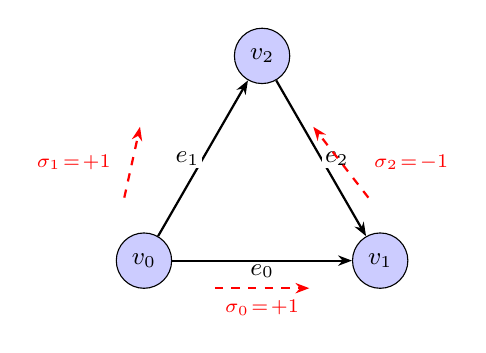
\begin{tikzpicture}[
  vertex/.style={circle, draw, fill=blue!20, minimum size=20pt, inner sep=0pt, font=\small},
  edge label/.style={font=\small, fill=white, inner sep=1pt},
  >={Stealth[length=5pt]}
]
  % Vertices: equilateral triangle, v0 at left, v1 at right, v2 at top
  \node[vertex] (v0) at (0, 0)     {$v_0$};
  \node[vertex] (v1) at (3, 0)     {$v_1$};
  \node[vertex] (v2) at (1.5, 2.6) {$v_2$};

  % Edge e0: v0 -> v1 (bottom)
  \draw[->, thick] (v0) -- node[edge label, below] {$e_0$} (v1);
  % Edge e1: v0 -> v2 (left)
  \draw[->, thick] (v0) -- node[edge label, left]  {$e_1$} (v2);
  % Edge e2: v2 -> v1 (right)
  \draw[->, thick] (v2) -- node[edge label, right] {$e_2$} (v1);

  % Spin arrows (offset from edges, showing sigma = (+1,+1,-1))
  % e0: sigma=+1, same as reference (v0->v1)
  \draw[->, red, thick, dashed] (0.9, -0.35) -- (2.1, -0.35);
  \node[red, font=\scriptsize] at (1.5, -0.6) {$\sigma_0\!=\!+1$};
  % e1: sigma=+1, same as reference (v0->v2)
  \draw[->, red, thick, dashed] (-0.25, 0.8) -- (-0.05, 1.7);
  \node[red, font=\scriptsize, left] at (-0.3, 1.25) {$\sigma_1\!=\!+1$};
  % e2: sigma=-1, opposes reference, so physical flow is v1->v2
  \draw[->, red, thick, dashed] (2.85, 0.8) -- (2.15, 1.7);
  \node[red, font=\scriptsize, right] at (2.8, 1.25) {$\sigma_2\!=\!-1$};
\end{tikzpicture}
\caption{Triangle $K_3$ with reference orientations (black arrows) and spin
configuration $\bm\sigma = (+1,+1,-1)^T$ (red dashed arrows showing physical
spin direction).  Vertex $v_0$ is a source ($Q=-2$), $v_1$ satisfies the
ice rule ($Q=0$), and $v_2$ is a sink ($Q=+2$).}
\label{fig:triangle}
\end{figure}

The incidence matrix is
\begin{equation}
  B_1 = \begin{pmatrix}
    -1 & -1 &  0 \\
    +1 &  0 & +1 \\
     0 & +1 & -1
  \end{pmatrix}
  \quad
  \begin{array}{l}
    \leftarrow v_0 \\ \leftarrow v_1 \\ \leftarrow v_2
  \end{array}
  \label{eq:B1_triangle}
\end{equation}
with columns indexed by $e_0, e_1, e_2$.  Each column has one $+1$ (head)
and one $-1$ (tail), and every column sums to zero.

Choose the spin configuration $\bm\sigma = (+1,\,+1,\,-1)^T$: spins on
$e_0$ and $e_1$ align with the reference orientation (pointing away from
$v_0$), while the spin on $e_2$ opposes it (pointing $v_1 \to v_2$).
This is a ``source'' configuration at $v_0$.

\subsection{\texorpdfstring{$S_{vv'}$}{S} matrix (Key Result~\ref{kr:S_matrix})}

Using $S_{ww'} = -[B_1]_{w,e}\,\sigma_e$ for adjacent $w, w'$ sharing
edge~$e$:
\begin{align*}
  S_{v_0 v_1} &= -[B_1]_{v_0,e_0}\,\sigma_{e_0}
  = -(-1)(+1) = +1, \\
  S_{v_0 v_2} &= -[B_1]_{v_0,e_1}\,\sigma_{e_1}
  = -(-1)(+1) = +1, \\
  S_{v_2 v_1} &= -[B_1]_{v_2,e_2}\,\sigma_{e_2}
  = -(-1)(-1) = -1.
\end{align*}
By antisymmetry, the full matrix is
\begin{equation}
  S = \begin{pmatrix}
     0 & +1 & +1 \\
    -1 &  0 & +1 \\
    -1 & -1 &  0
  \end{pmatrix}.
\end{equation}

\paragraph{Matrix-formula verification.}
We verify~\eqref{eq:Smatrix} by computing
$M = |B_1|\,D_\sigma\,B_1^T$ where $D_\sigma = \diag(+1,+1,-1)$:
\begin{equation}
  |B_1| = \begin{pmatrix}
    1 & 1 & 0 \\ 1 & 0 & 1 \\ 0 & 1 & 1
  \end{pmatrix},
  \quad
  D_\sigma B_1^T = \begin{pmatrix}
    -1 & +1 &  0 \\
    -1 &  0 & +1 \\
     0 & -1 & +1
  \end{pmatrix}.
\end{equation}
Then $M = |B_1|\,(D_\sigma B_1^T)$:
\begin{equation}
  M = \begin{pmatrix}
    -2 & +1 & +1 \\
    -1 &  0 & +1 \\
    -1 & -1 & +2
  \end{pmatrix}.
\end{equation}
The diagonal gives the charges:
$\diag(M) = (-2,\,0,\,+2) = \mathbf{Q}$.
The skew-symmetrization $\tfrac{1}{2}(M - M^T) = S$.~$\checkmark$

\subsection{Topological charge (Key Result~\ref{kr:charge})}

\begin{equation}
  \mathbf{Q} = B_1\bm\sigma
  = \begin{pmatrix} -1-1+0 \\ +1+0-1 \\ 0+1+1 \end{pmatrix}
  = \begin{pmatrix} -2 \\ 0 \\ +2 \end{pmatrix}.
\end{equation}
$v_0$ is a negative monopole (source, $Q = -2$); $v_1$ satisfies the ice
rule ($Q = 0$); $v_2$ is a positive monopole (sink, $Q = +2$).  Total
charge: $\sum_v Q_v = 0$.~$\checkmark$

\paragraph{Ice manifold.}
$\dim(\ker B_1) = n_1 - n_0 + 1 = 1$.  A basis vector is
$\bm\sigma_{\text{ice}} = (+1,\,-1,\,-1)^T$ (a clockwise circulation:
$v_0 \to v_1 \to v_2 \to v_0$, every vertex has one spin in and one out).
The full ice manifold on $K_3$ is
$\calI = \{(+1,-1,-1),\;(-1,+1,+1)\}$---the two circulations.

\paragraph{Coulomb classes.}
$K_3$ has $2^3 = 8$ spin configurations partitioned into four Coulomb
classes:
$C_{\mathbf{0}} = \{(\pm 1,\mp 1,\mp 1)\}$ (two ice states),
and three monopole classes of two configurations each.

\subsection{Hamiltonian (Key Result~\ref{kr:hamiltonian})}

\begin{equation}
  L_1^{\text{down}} = B_1^T B_1
  = \begin{pmatrix} 2 & 1 & 1 \\ 1 & 2 & -1 \\ 1 & -1 & 2 \end{pmatrix}.
\end{equation}

\textbf{Non-ice configuration} $\bm\sigma = (+1,+1,-1)^T$
($\mathbf{Q} = (-2,0,+2)^T$):
\begin{equation}
  \bm\sigma^T L_1^{\text{down}}\bm\sigma
  = \|\mathbf{Q}\|^2 = 4 + 0 + 4 = 8,
  \qquad
  \calH = \tfrac{\epsilon}{2}\cdot 8 = 4\epsilon.
\end{equation}

\textbf{Ice configuration} $\bm\sigma_{\text{ice}} = (+1,-1,-1)^T$:
\begin{equation}
  B_1\bm\sigma_{\text{ice}} = \mathbf{0},
  \qquad
  \calH_{\text{ice}} = 0.\;\checkmark
\end{equation}

\textbf{Spectrum of $L_1^{\text{down}}$.}  The eigenvalues are
$\{0, 3, 3\}$: one zero eigenvalue ($\beta_1 = 1$, the ice manifold) and
a doubly-degenerate spectral gap $\Delta = 3$.  The minimum monopole pair
energy is $\calH_{\min} = (\epsilon/2)\cdot\Delta\cdot c_{\min}^2$ where
$c_{\min}^2$ is the smallest nonzero squared expansion coefficient.


% -------------------------------------------------------------------
\section{Worked Example: \texorpdfstring{$3\times 3$}{3x3} Periodic Square Lattice}
\label{app:torus}

This appendix works through the full computation on a $3\times 3$ square
lattice with periodic boundary conditions (a discrete torus), producing
every matrix and eigenvalue explicitly.

\subsection{Lattice setup}

\textbf{Vertices:} 9 vertices on a $3\times 3$ grid, labeled $v_0,\ldots,v_8$
in row-major order with coordinates $v_k$ at
$(k\bmod 3,\;\lfloor k/3\rfloor)$.

\textbf{Periodic BCs:} Right wraps to left
($v_2 \sim v_0$, $v_5 \sim v_3$, $v_8 \sim v_6$);
top wraps to bottom
($v_6 \sim v_0$, $v_7 \sim v_1$, $v_8 \sim v_2$).
Topologically a torus~$T^2$.

\textbf{Edges:} $n_1 = 18$ (9~horizontal $+$ 9~vertical).
Reference orientation: horizontal edges point right, vertical edges point up.
Wrap-around edges: $e_2 (v_2\!\to\!v_0)$, $e_5 (v_5\!\to\!v_3)$,
$e_8 (v_8\!\to\!v_6)$, $e_{15} (v_6\!\to\!v_0)$,
$e_{16} (v_7\!\to\!v_1)$, $e_{17} (v_8\!\to\!v_2)$.

\textbf{Faces:} $n_2 = 9$ unit squares, all oriented counterclockwise.

\textbf{Counts:} $n_0 = 9$, $n_1 = 18$, $n_2 = 9$.  All vertices have
coordination $z_v = 4$.

\begin{figure}[h]
\centering
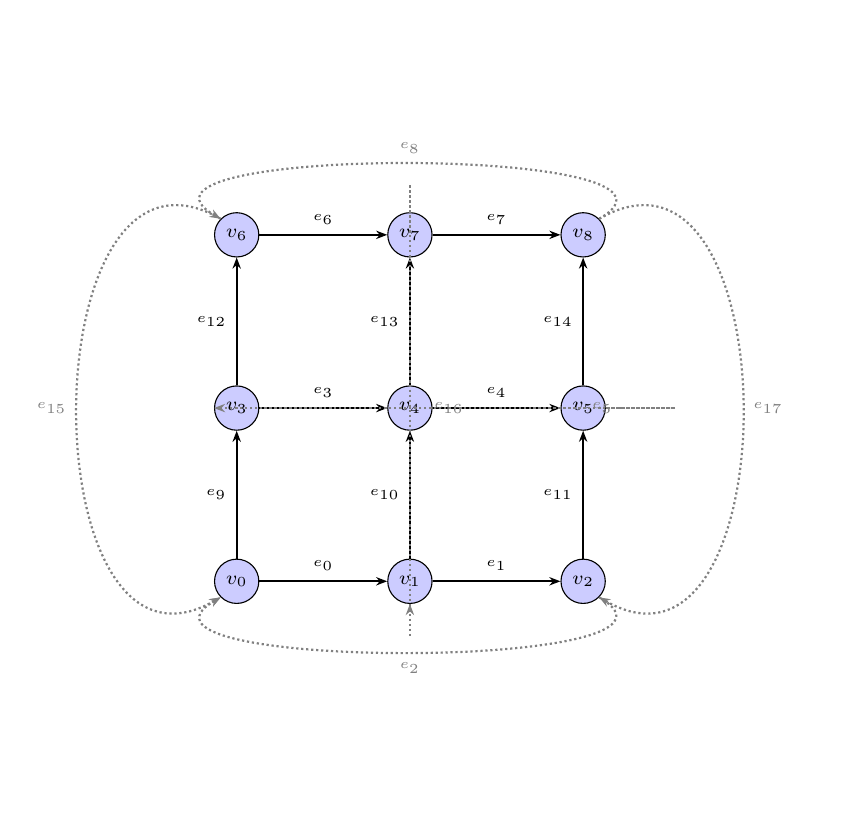
\begin{tikzpicture}[
  vertex/.style={circle, draw, fill=blue!20, minimum size=16pt, inner sep=0pt, font=\scriptsize},
  wrap/.style={->, thick, densely dotted, gray},
  >={Stealth[length=4pt]},
  scale=1.0
]
  % Grid spacing
  \def\s{2.2}

  % Vertices: row-major v0..v8
  \foreach \r in {0,1,2} {
    \foreach \c in {0,1,2} {
      \pgfmathtruncatemacro{\idx}{\r*3+\c}
      \node[vertex] (v\idx) at (\c*\s, \r*\s) {$v_{\idx}$};
    }
  }

  % Horizontal edges (reference: right)
  % Row 0: e0(v0->v1), e1(v1->v2), e2(v2->v0 wrap)
  \draw[->, thick] (v0) -- node[font=\tiny, above] {$e_0$} (v1);
  \draw[->, thick] (v1) -- node[font=\tiny, above] {$e_1$} (v2);
  % Row 1: e3(v3->v4), e4(v4->v5), e5(v5->v3 wrap)
  \draw[->, thick] (v3) -- node[font=\tiny, above] {$e_3$} (v4);
  \draw[->, thick] (v4) -- node[font=\tiny, above] {$e_4$} (v5);
  % Row 2: e6(v6->v7), e7(v7->v8), e8(v8->v6 wrap)
  \draw[->, thick] (v6) -- node[font=\tiny, above] {$e_6$} (v7);
  \draw[->, thick] (v7) -- node[font=\tiny, above] {$e_7$} (v8);

  % Vertical edges (reference: up)
  % Col 0: e9(v0->v3), e12(v3->v6), e15(v6->v0 wrap)
  \draw[->, thick] (v0) -- node[font=\tiny, left] {$e_9$} (v3);
  \draw[->, thick] (v3) -- node[font=\tiny, left] {$e_{12}$} (v6);
  % Col 1: e10(v1->v4), e13(v4->v7), e16(v7->v1 wrap)
  \draw[->, thick] (v1) -- node[font=\tiny, left] {$e_{10}$} (v4);
  \draw[->, thick] (v4) -- node[font=\tiny, left] {$e_{13}$} (v7);
  % Col 2: e11(v2->v5), e14(v5->v8), e17(v8->v2 wrap)
  \draw[->, thick] (v2) -- node[font=\tiny, left] {$e_{11}$} (v5);
  \draw[->, thick] (v5) -- node[font=\tiny, left] {$e_{14}$} (v8);

  % Wrap-around horizontal edges (dotted, curving outside the grid)
  % e2: v2 -> v0 (right wraps to left, row 0)
  \draw[wrap] (v2.south east) to[out=-30, in=-150]
    node[font=\tiny, below] {$e_2$} (v0.south west);
  % e5: v5 -> v3 (row 1)
  \draw[wrap] (v5.east) to[out=0, in=0, looseness=1.5]
    node[font=\tiny, right] {$e_5$} (v3.west);
  % e8: v8 -> v6 (row 2)
  \draw[wrap] (v8.north east) to[out=30, in=150]
    node[font=\tiny, above] {$e_8$} (v6.north west);

  % Wrap-around vertical edges (dotted, curving outside the grid)
  % e15: v6 -> v0 (top wraps to bottom, col 0)
  \draw[wrap] (v6.north west) to[out=150, in=-150, looseness=1.5]
    node[font=\tiny, left] {$e_{15}$} (v0.south west);
  % e16: v7 -> v1 (col 1)
  \draw[wrap] (v7.north) to[out=90, in=-90, looseness=1.2]
    node[font=\tiny, right, xshift=5pt] {$e_{16}$} (v1.south);
  % e17: v8 -> v2 (col 2)
  \draw[wrap] (v8.north east) to[out=30, in=-30, looseness=1.5]
    node[font=\tiny, right] {$e_{17}$} (v2.south east);

\end{tikzpicture}
\caption{The $3\times 3$ periodic square lattice (torus $T^2$).  Solid arrows
show the 12~interior edges with reference orientations (horizontal: right,
vertical: up).  Dotted gray arrows show the 6~wrap-around edges implementing
periodic boundary conditions.  Vertices are labeled $v_0$--$v_8$ in row-major
order.}
\label{fig:torus}
\end{figure}

\subsection{Incidence matrix \texorpdfstring{$B_1$}{B1} \texorpdfstring{$(9\times 18)$}{(9x18)}}

Using the convention $[B_1]_{v,e} = +1$ at the head, $-1$ at the tail:

{\small
\begin{equation}
B_1 = \left(\begin{array}{@{}rrrrrrrrrrrrrrrrrr@{}}
-1 &  0 &  1 &  0 &  0 &  0 &  0 &  0 &  0 & -1 &  0 &  0 &  0 &  0 &  0 &  1 &  0 &  0 \\
 1 & -1 &  0 &  0 &  0 &  0 &  0 &  0 &  0 &  0 & -1 &  0 &  0 &  0 &  0 &  0 &  1 &  0 \\
 0 &  1 & -1 &  0 &  0 &  0 &  0 &  0 &  0 &  0 &  0 & -1 &  0 &  0 &  0 &  0 &  0 &  1 \\
 0 &  0 &  0 & -1 &  0 &  1 &  0 &  0 &  0 &  1 &  0 &  0 & -1 &  0 &  0 &  0 &  0 &  0 \\
 0 &  0 &  0 &  1 & -1 &  0 &  0 &  0 &  0 &  0 &  1 &  0 &  0 & -1 &  0 &  0 &  0 &  0 \\
 0 &  0 &  0 &  0 &  1 & -1 &  0 &  0 &  0 &  0 &  0 &  1 &  0 &  0 & -1 &  0 &  0 &  0 \\
 0 &  0 &  0 &  0 &  0 &  0 & -1 &  0 &  1 &  0 &  0 &  0 &  1 &  0 &  0 & -1 &  0 &  0 \\
 0 &  0 &  0 &  0 &  0 &  0 &  1 & -1 &  0 &  0 &  0 &  0 &  0 &  1 &  0 &  0 & -1 &  0 \\
 0 &  0 &  0 &  0 &  0 &  0 &  0 &  1 & -1 &  0 &  0 &  0 &  0 &  0 &  1 &  0 &  0 & -1
\end{array}\right)
\label{eq:B1_torus}
\end{equation}
}

Each column has one $+1$ and one $-1$; each row has four nonzero entries
(two $+1$, two $-1$) reflecting $z_v = 4$.

\subsection{Incidence matrix \texorpdfstring{$B_2$}{B2} \texorpdfstring{$(18\times 9)$}{(18x9)}}

For face~$f_j$ with CCW boundary, $[B_2]_{e,f} = +1$ if edge~$e$ is
traversed in its reference direction, $-1$ if against.  For example,
$f_0$ has boundary $+e_0,+e_{10},-e_3,-e_9$:

{\small
\begin{equation}
B_2 = \left(\begin{array}{@{}rrrrrrrrr@{}}
 1 &  0 &  0 &  0 &  0 &  0 & -1 &  0 &  0 \\
 0 &  1 &  0 &  0 &  0 &  0 &  0 & -1 &  0 \\
 0 &  0 &  1 &  0 &  0 &  0 &  0 &  0 & -1 \\
-1 &  0 &  0 &  1 &  0 &  0 &  0 &  0 &  0 \\
 0 & -1 &  0 &  0 &  1 &  0 &  0 &  0 &  0 \\
 0 &  0 & -1 &  0 &  0 &  1 &  0 &  0 &  0 \\
 0 &  0 &  0 & -1 &  0 &  0 &  1 &  0 &  0 \\
 0 &  0 &  0 &  0 & -1 &  0 &  0 &  1 &  0 \\
 0 &  0 &  0 &  0 &  0 & -1 &  0 &  0 &  1 \\
-1 &  0 &  1 &  0 &  0 &  0 &  0 &  0 &  0 \\
 1 & -1 &  0 &  0 &  0 &  0 &  0 &  0 &  0 \\
 0 &  1 & -1 &  0 &  0 &  0 &  0 &  0 &  0 \\
 0 &  0 &  0 & -1 &  0 &  1 &  0 &  0 &  0 \\
 0 &  0 &  0 &  1 & -1 &  0 &  0 &  0 &  0 \\
 0 &  0 &  0 &  0 &  1 & -1 &  0 &  0 &  0 \\
 0 &  0 &  0 &  0 &  0 &  0 & -1 &  0 &  1 \\
 0 &  0 &  0 &  0 &  0 &  0 &  1 & -1 &  0 \\
 0 &  0 &  0 &  0 &  0 &  0 &  0 &  1 & -1
\end{array}\right)
\label{eq:B2_torus}
\end{equation}
}

Each column (face) has four nonzero entries; each row (edge) appears in
exactly two faces.

\subsection{Verification: \texorpdfstring{$B_1 B_2 = 0$}{B1 B2 = 0}}

We verify on face~$f_0$ (first column of $B_2$, nonzero at
$e_0 (+1)$, $e_3 (-1)$, $e_9 (-1)$, $e_{10} (+1)$).
For each vertex:
\begin{align*}
  v_0 &: (-1)(+1) + 0(-1) + (-1)(-1) + 0(+1) = -1+1 = 0, \\
  v_1 &: (+1)(+1) + 0(-1) + 0(-1) + (-1)(+1) = 1-1 = 0, \\
  v_3 &: 0(+1) + (-1)(-1) + (+1)(-1) + 0(+1) = 1-1 = 0, \\
  v_4 &: 0(+1) + (+1)(-1) + 0(-1) + (+1)(+1) = -1+1 = 0.
\end{align*}
All other vertices have no incident edges in~$f_0$.
The same holds for all columns: $B_1 B_2 = 0$.~$\checkmark$

\subsection{Graph Laplacian \texorpdfstring{$L_0$}{L0} and its spectrum}

With $z_v = 4$ everywhere, $L_0 = 4I_9 - A$.  The eigenvalues of the
$3\times 3$ torus are
\begin{equation}
  \lambda_{jk} = 2\bigl(2 - \cos(2\pi j/3) - \cos(2\pi k/3)\bigr),
  \quad j,k \in \{0,1,2\},
\end{equation}
giving spectrum $\{0,\, 3^{(\times 4)},\, 6^{(\times 4)}\}$.
Spectral gap $\lambda_1 = 3$; one zero eigenvalue confirms
$\beta_0 = 1$.~$\checkmark$

\subsection{Betti numbers and Euler characteristic}

Expected for the torus $T^2$: $\beta_0 = 1$, $\beta_1 = 2$, $\beta_2 = 1$.

\textbf{Euler characteristic:}
\begin{equation}
  \chi = n_0 - n_1 + n_2 = 9 - 18 + 9 = 0
  = \beta_0 - \beta_1 + \beta_2 = 1 - 2 + 1.\;\checkmark
\end{equation}

\textbf{Rank check:}
\begin{equation}
  \beta_1 = n_1 - \rank(B_1) - \rank(B_2) = 18 - 8 - 8 = 2.\;\checkmark
\end{equation}

\textbf{Ice manifold dimension:}
$\dim(\ker B_1) = 18 - 8 = 10$, which splits as
$\rank(B_2) + \beta_1 = 8 + 2 = 10$.~$\checkmark$

\subsection{Spectrum of \texorpdfstring{$L_1$}{L1}}

The eigenvalues of $L_1^{\text{down}} = B_1^T B_1$ on $\R^{18}$:
\begin{equation}
  \{0^{(\times 10)},\; 3^{(\times 4)},\; 6^{(\times 4)}\}.
\end{equation}
The 10 zero eigenvalues span $\ker(B_1)$ (the ice manifold).  The nonzero
eigenvalues match those of $L_0$ (standard property: $B_1^T B_1$ and
$B_1 B_1^T$ share nonzero spectra).

The eigenvalues of $L_1^{\text{up}} = B_2 B_2^T$ on $\R^{18}$:
\begin{equation}
  \{0^{(\times 10)},\; 3^{(\times 4)},\; 6^{(\times 4)}\}.
\end{equation}

The combined Hodge 1-Laplacian $L_1 = L_1^{\text{down}} + L_1^{\text{up}}$:
\begin{equation}
  \operatorname{spec}(L_1)
  = \{\underbrace{0,\, 0}_{\beta_1 = 2},\;
      \underbrace{3,3,3,3,3,3,3,3}_{8},\;
      \underbrace{6,6,6,6,6,6,6,6}_{8}\}.
\end{equation}
Spectral gap $\Delta_1 = 3$.

\subsection{The two harmonic modes}

The two harmonic eigenvectors $\mathbf{h}_H, \mathbf{h}_V \in \ker(L_1)$
correspond to the two non-contractible cycles on the torus:

\textbf{Horizontal winding mode:}
$[\mathbf{h}_H]_e = 1/3$ for horizontal edges, $0$ for vertical.
(Normalized: $\|\mathbf{h}_H\|^2 = 9\cdot(1/3)^2 = 1$.)

\textbf{Vertical winding mode:}
$[\mathbf{h}_V]_e = 0$ for horizontal edges, $1/3$ for vertical.

Verification: $B_1\mathbf{h}_H = \mathbf{0}$ (at each vertex, one
horizontal edge enters and one leaves due to periodicity).
$B_2^T\mathbf{h}_H = \mathbf{0}$ (each face has one horizontal edge
traversed forward and one backward, canceling).  Therefore
$L_1\mathbf{h}_H = \mathbf{0}$.~$\checkmark$

These two modes are orthogonal and span $\ker(L_1)$.  They represent
topologically protected degrees of freedom: no sequence of local plaquette
flips can change the winding numbers.

\subsection{Ice configuration and Hodge decomposition}

The ``all-right, all-up'' configuration has
$\bm\sigma_0 = (1,1,1,1,1,1,1,1,1,\;1,1,1,1,1,1,1,1,1)^T$.

\textbf{Ice rule:} At each vertex, two edges point in and two point out,
so $B_1\bm\sigma_0 = \mathbf{0}$.~$\checkmark$

\textbf{Hodge projection:}
$\langle\bm\sigma_0, \mathbf{h}_H\rangle = 9\cdot(1/3) = 3$,\;
$\langle\bm\sigma_0, \mathbf{h}_V\rangle = 3$.  So
$\bm\sigma_{\text{harm}} = 3\mathbf{h}_H + 3\mathbf{h}_V = \bm\sigma_0$.
The curl component is $\bm\sigma_{\text{curl}} = \mathbf{0}$: this
configuration is \emph{purely harmonic}.  It has nonzero winding number in
both directions and no local curl structure.

\subsection{A monopole excitation}

Starting from $\bm\sigma_0$, flip $e_0$ ($v_0 \to v_1$):
set $\sigma_{e_0} = -1$.  Call this $\bm\sigma_1$.
\begin{equation}
  \mathbf{Q} = B_1\bm\sigma_1
  = B_1\bm\sigma_0 - 2\,B_1\mathbf{e}_0
  = -2\begin{pmatrix} -1\\1\\0\\\cdots\\0 \end{pmatrix}
  = \begin{pmatrix} +2\\-2\\0\\\cdots\\0 \end{pmatrix}.
\end{equation}
A monopole--antimonopole pair: $Q_{v_0} = +2$, $Q_{v_1} = -2$, all others
zero.

\textbf{Energy:}
$\calH[\bm\sigma_1] = (\epsilon/2)\|\mathbf{Q}\|^2 = (\epsilon/2)(4+4)
= 4\epsilon$.  The ice configuration had $\calH = 0$, so the monopole
pair costs~$4\epsilon$.

\subsection{Pauling entropy}

The Pauling approximation for uniform $z = 4$:
\begin{equation}
  |\calI_{\text{P}}|
  = 2^{18}\!\left(\frac{\binom{4}{2}}{2^4}\right)^{\!9}
  = 2^{18}\!\left(\frac{3}{8}\right)^{\!9}
  \approx 38.4.
\end{equation}
Pauling entropy per vertex:
$s_{\text{P}} = \frac{1}{9}\ln 38.4 \approx 0.405$,
close to Lieb's exact result~\cite{lieb1967}
$s_{\text{Lieb}} = \tfrac{3}{2}\ln(4/3) \approx 0.431$.
The small discrepancy is a finite-size effect.

\subsection{Loop basis and reachable states}

With no faces filled ($n_2 = 0$):
$\beta_1 = \dim(\ker B_1) = 18 - 9 + 1 = 10$,
giving an upper bound of $2^{10} = 1024$ from the loop-flip
parameterization.  The Pauling estimate is $\approx 38$, so the ratio
$38/1024 \approx 3.7\%$ reflects severe directed-cycle pruning, consistent
with the patterns in \cref{tab:counting}.

With all 9 faces filled ($n_2 = 9$): the faces account for 8 of the 10
independent cycles (9~faces minus one linear relation), leaving
$\beta_1 = 10 - 8 = 2$.  The two surviving harmonic modes are exactly the
horizontal and vertical winding modes from the previous subsection---the
non-contractible cycles that wrap around the torus.  This illustrates the
two extremes of the face-filling strategy: with no faces, $\beta_1 = 10$
and the full cycle space is available for loop-flip sampling; with all
faces, $\beta_1 = 2$ and only the global winding modes survive.

\end{document}
